% !TEX root =  main.tex
\chapter{Modified PCA models}

\section{Heterogeneous Learning Rates}
To introduce learning rate heterogeneity in the classroom, we revisit equation \ref{eq:BPCA PI learning probability}. 
\begin{equation*}
    P_{ij} = 1 - \prod_{\forall \delta i, \delta j}{\lbrack1-(\lambda_{ij})(\rho_{i+\delta i, j+\delta j})(s_{i+\delta i, j+\delta j})}\rbrack
    \tag{\ref{eq:BPCA PI learning probability} revisted}
\end{equation*}
We can adjust the parameter $\lambda_{ij}$ to introduce differences in each student's learning rate. 
We set a student's learning rate as $\lambda_{ij} = \lambda_0 \pm \delta\lambda$ where $\delta\lambda \in \lbrace 0.0,0.1, 0.2, 0.3, 0.4\rbrace$ and $\lambda_0 = 0.5$. 
Each student has an equal chance of having a learning rate that is either faster $(\lambda_0 + \delta\lambda)$ or slower $(\lambda_0 - \delta\lambda)$ than the average learning rate $\lambda_0$. 

$\lambda_{i,j} \in [0,1]$ is the learning rate of student $c_{i,j}$ with values $\lambda_{i,j} = \lbrace \lambda_0 \pm \delta \lambda \rbrace$ where $\lambda_0 = 0.5$ and $\delta \lambda = \lbrace 0.1, 0.2, 0.3, 0.4 \rbrace$, 

\subsection{Effects on classroom evolution}\label{subsec:BPCAIH effects on classroom evolution}
As shown in the figures in this subsection, we notice values of $\rho_0$ is still the most important factor in determining $t_{max}$. 
However, irregularities in the shapes of the "wave of learning" become more pronounced for lower values of $\rho_0$ and high values of $\delta\lambda$ as shown in figure \ref{fig:2DBPCAIH sample class evolution low rho}.
These irregularities are also more pronounced at the start of the classroom.
We also notice that compared to the homogenous model, there is a more evident deviation from the power law at earlier times $t$.
The irregularities in both the shape of the "wave of learning" and the deviation from the power law are less pronounced for higher values of $\rho_0$, regardless of the value of $\delta\lambda$, as shown in figure \ref{fig:2DBPCAIH sample class evolution high rho} and \ref{fig:2DBPCAIH sample class evolution high rho high delta}.
For high values of $\rho_0$, high values of $\delta\lambda$ leads to the irregularity in the "wave of learning" to persist longer than those with lower values of $\delta\lambda$.

\begin{figure}[htbp!]
   \centering
   \subfigure[$t=48$]{\label{fig:2DBPCAIH class evolution low rho 48}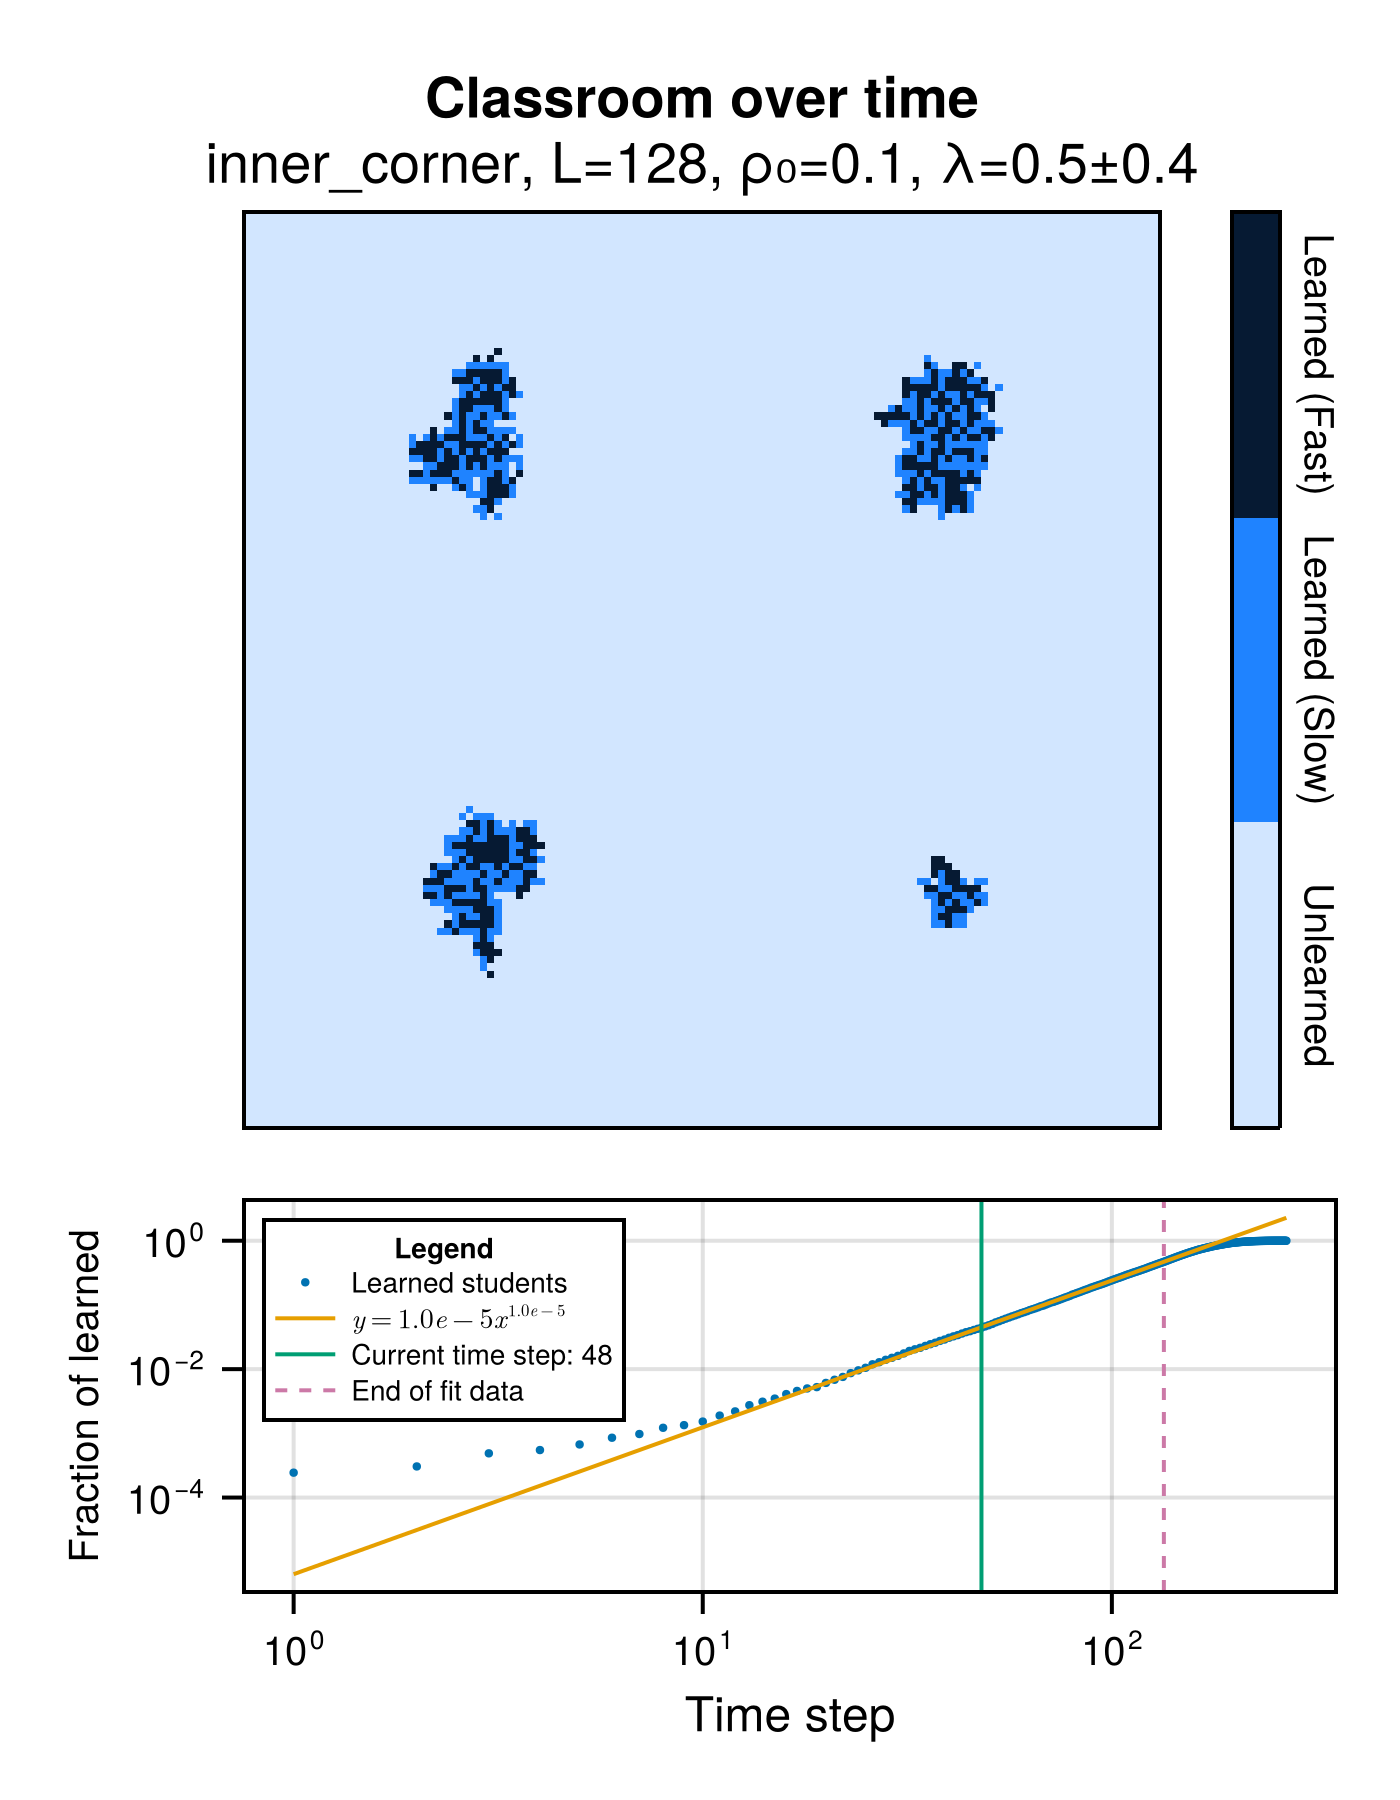
\includegraphics[width=0.49\textwidth]{figures/2D-BPCAIH-analysis/class evolutions/low rho/2DBPCAIH-inner_corner-128-0.1-0.5-0.4-trial_3-48.png}}
   \subfigure[$t=69$]{\label{fig:2DBPCAIH class evolution low rho 69}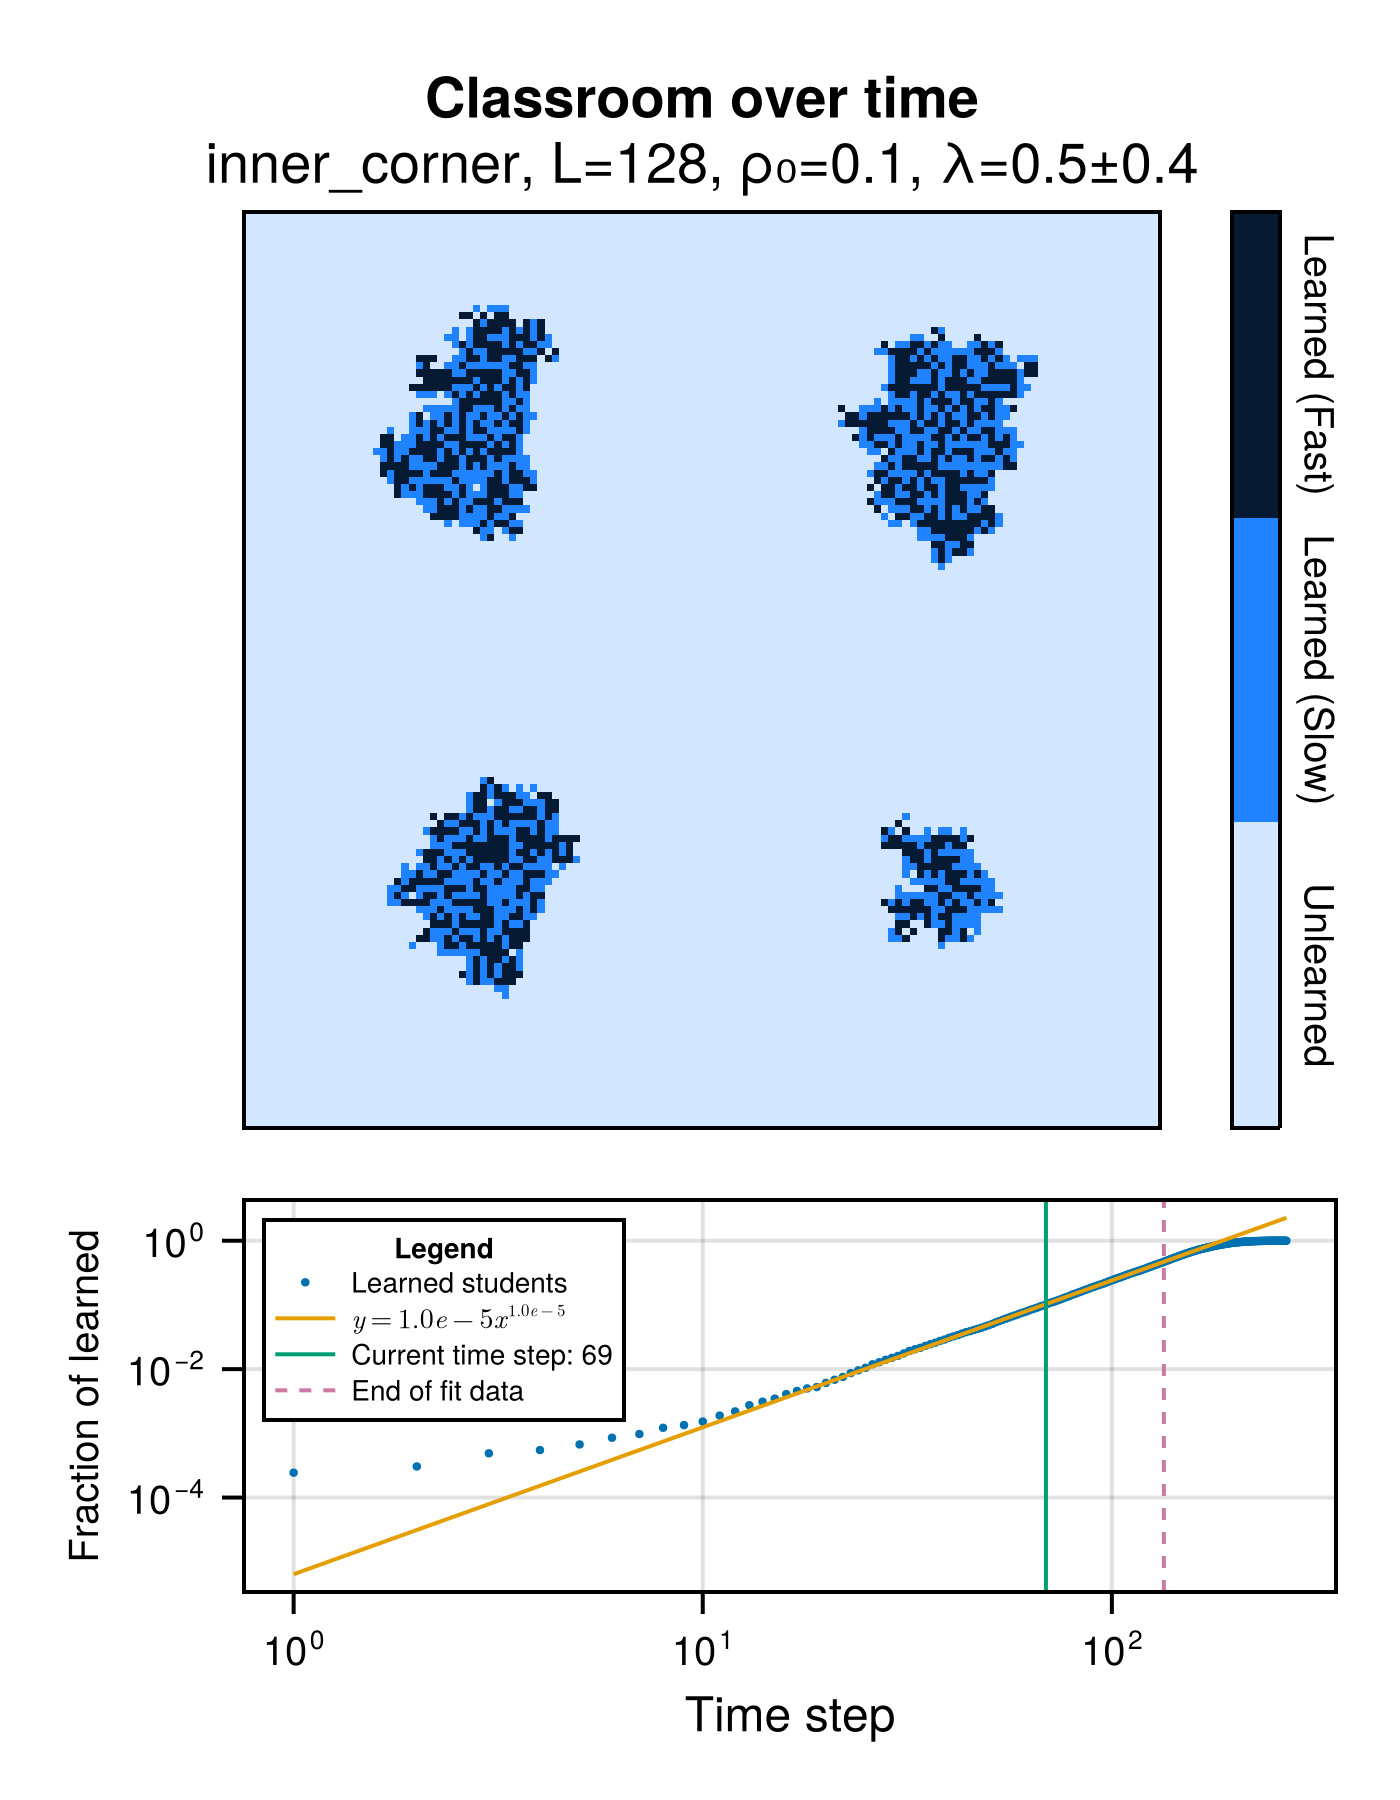
\includegraphics[width=0.49\textwidth]{figures/2D-BPCAIH-analysis/class evolutions/low rho/2DBPCAIH-inner_corner-128-0.1-0.5-0.4-trial_3-69.png}}
   \subfigure[$t=128$]{\label{fig:2DBPCAIH class evolution low rho 128}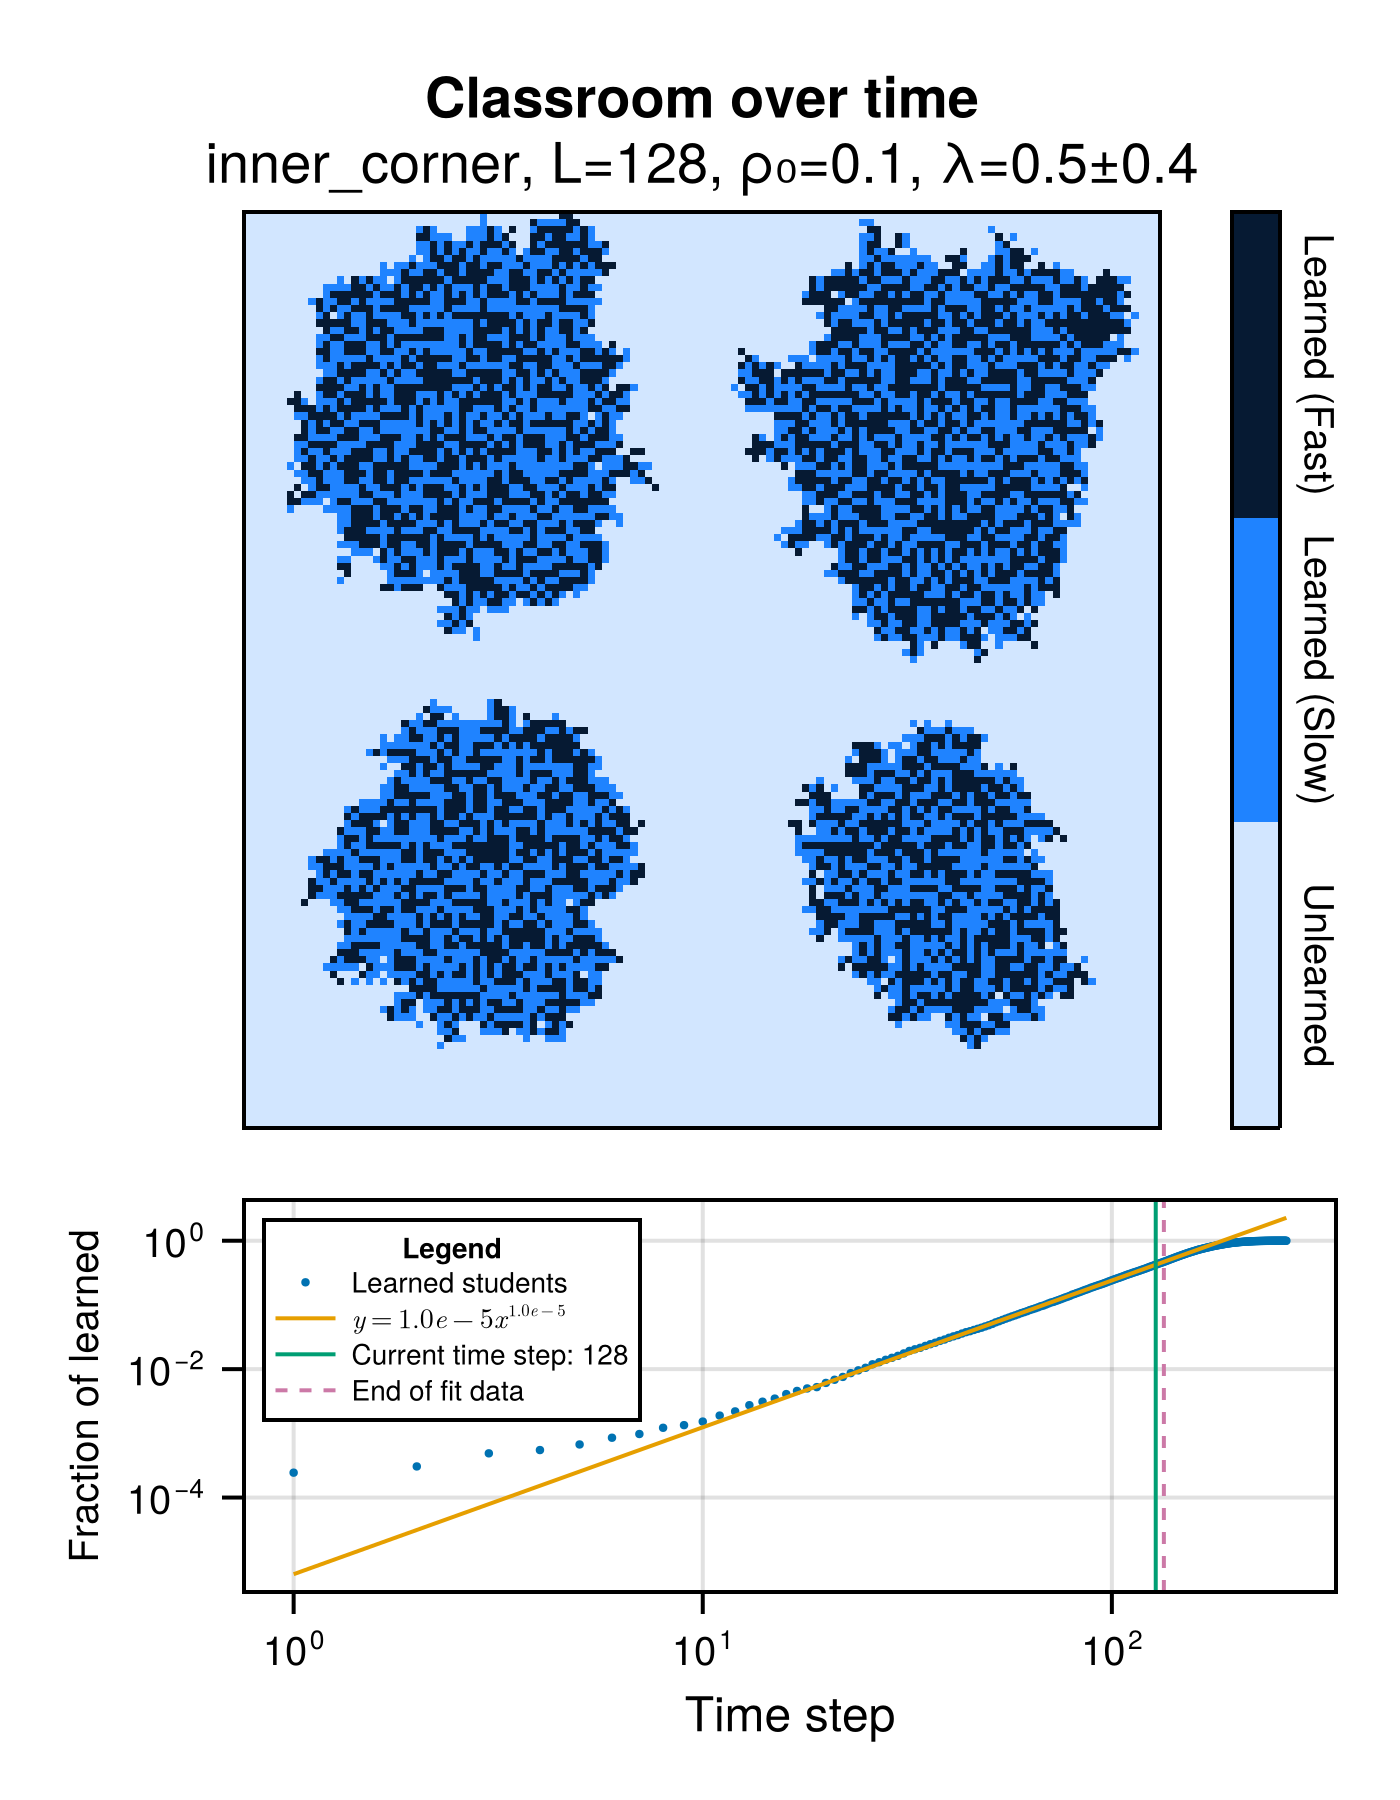
\includegraphics[width=0.49\textwidth]{figures/2D-BPCAIH-analysis/class evolutions/low rho/2DBPCAIH-inner_corner-128-0.1-0.5-0.4-trial_3-128.png}}
   \subfigure[$t=200$]{\label{fig:2DBPCAIH class evolution low rho 200}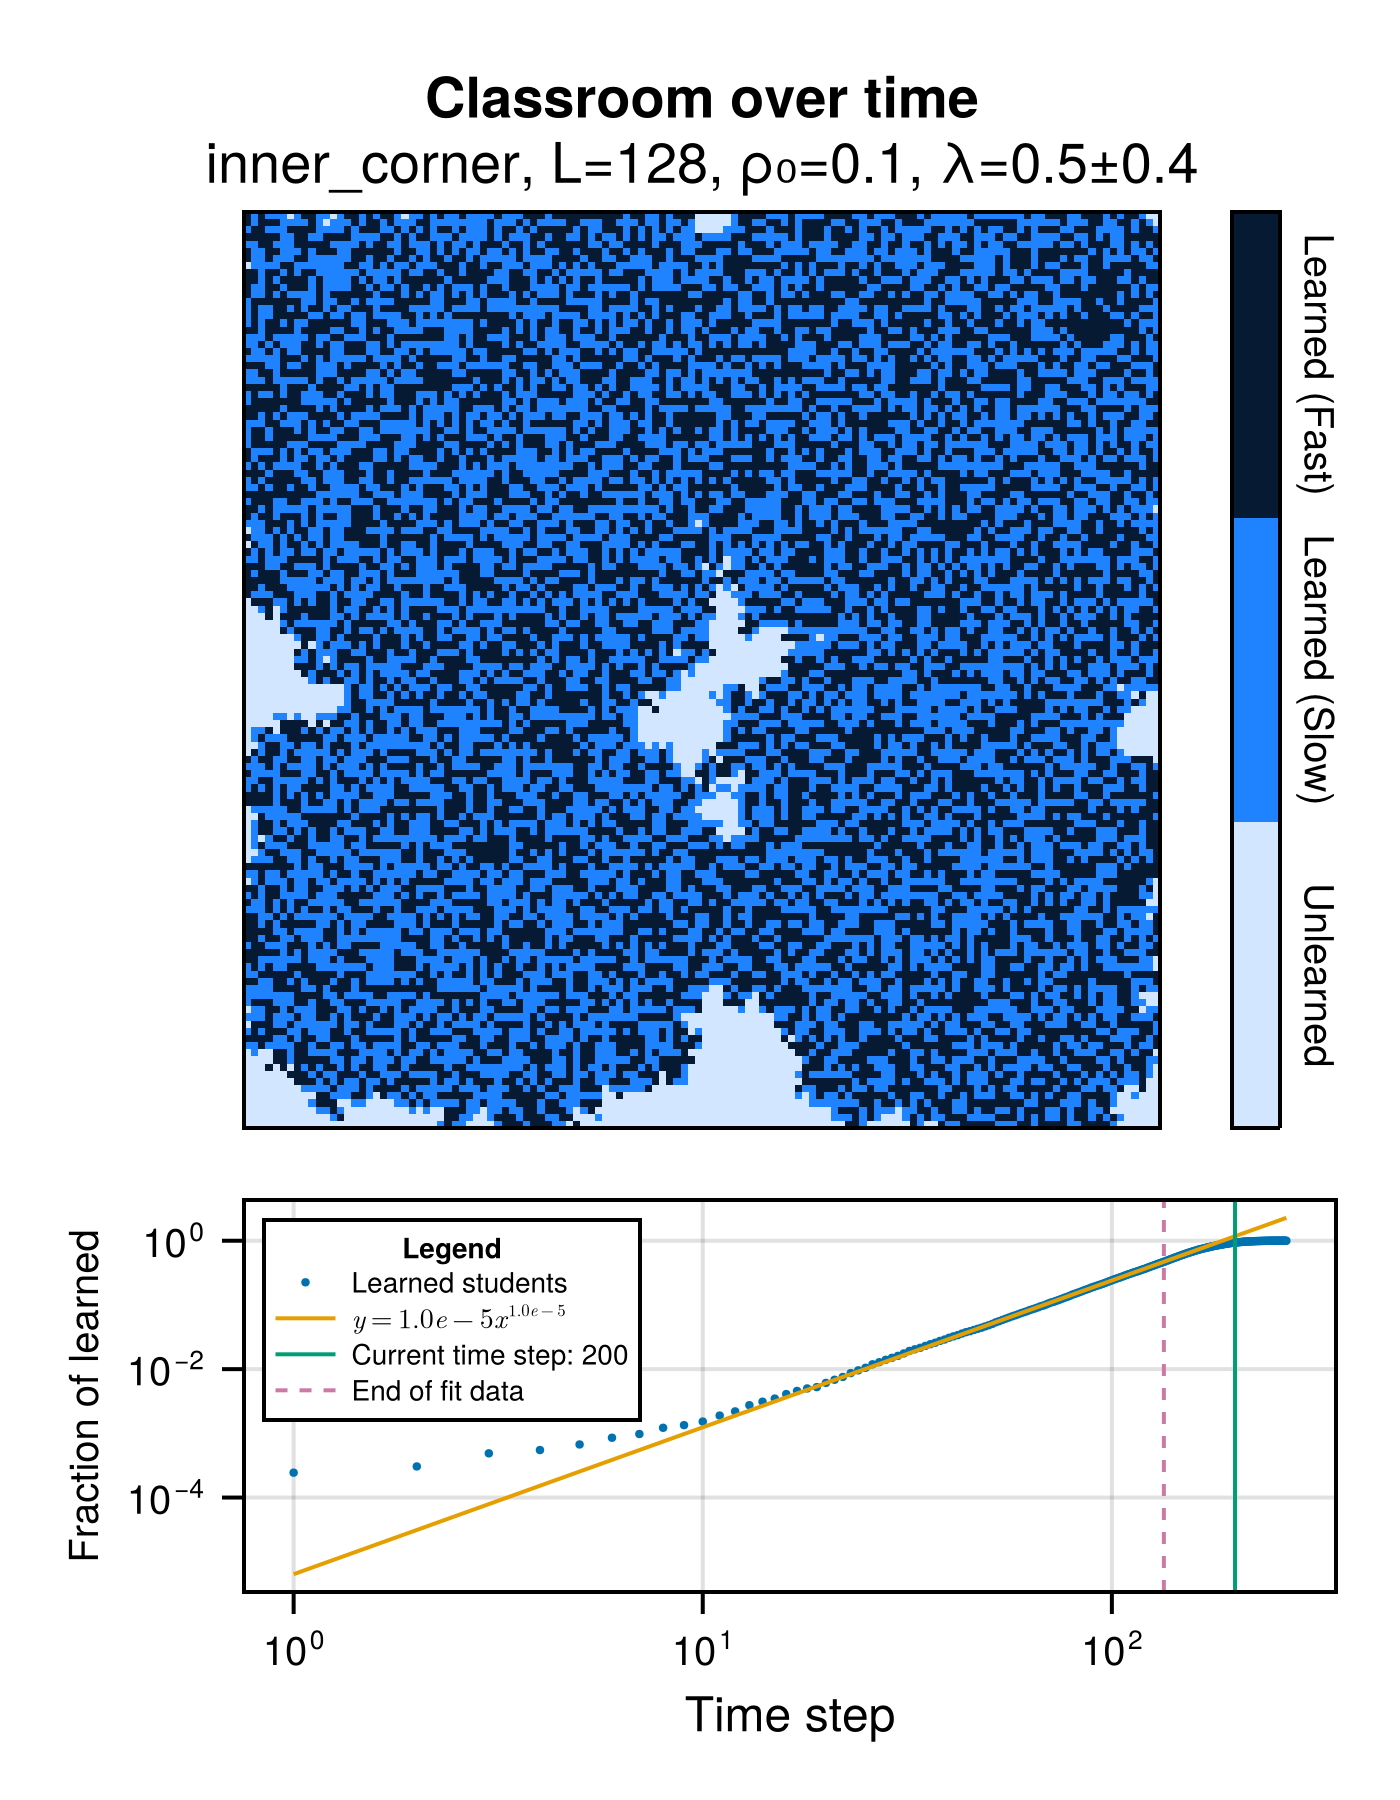
\includegraphics[width=0.49\textwidth]{figures/2D-BPCAIH-analysis/class evolutions/low rho/2DBPCAIH-inner_corner-128-0.1-0.5-0.4-trial_3-200.png}}
   \caption{Sample classroom evolutions for the inner corner configuration with $L=128$ at different times $t$ for positional learning rate $\rho_0=0.1$, $\delta\lambda = 0.4$.}
   \label{fig:2DBPCAIH sample class evolution low rho}
 \end{figure}

 \begin{figure}[htbp!]
    \centering
    \subfigure[$t=5$]{\label{fig:2DBPCAIH class evolution high rho 5}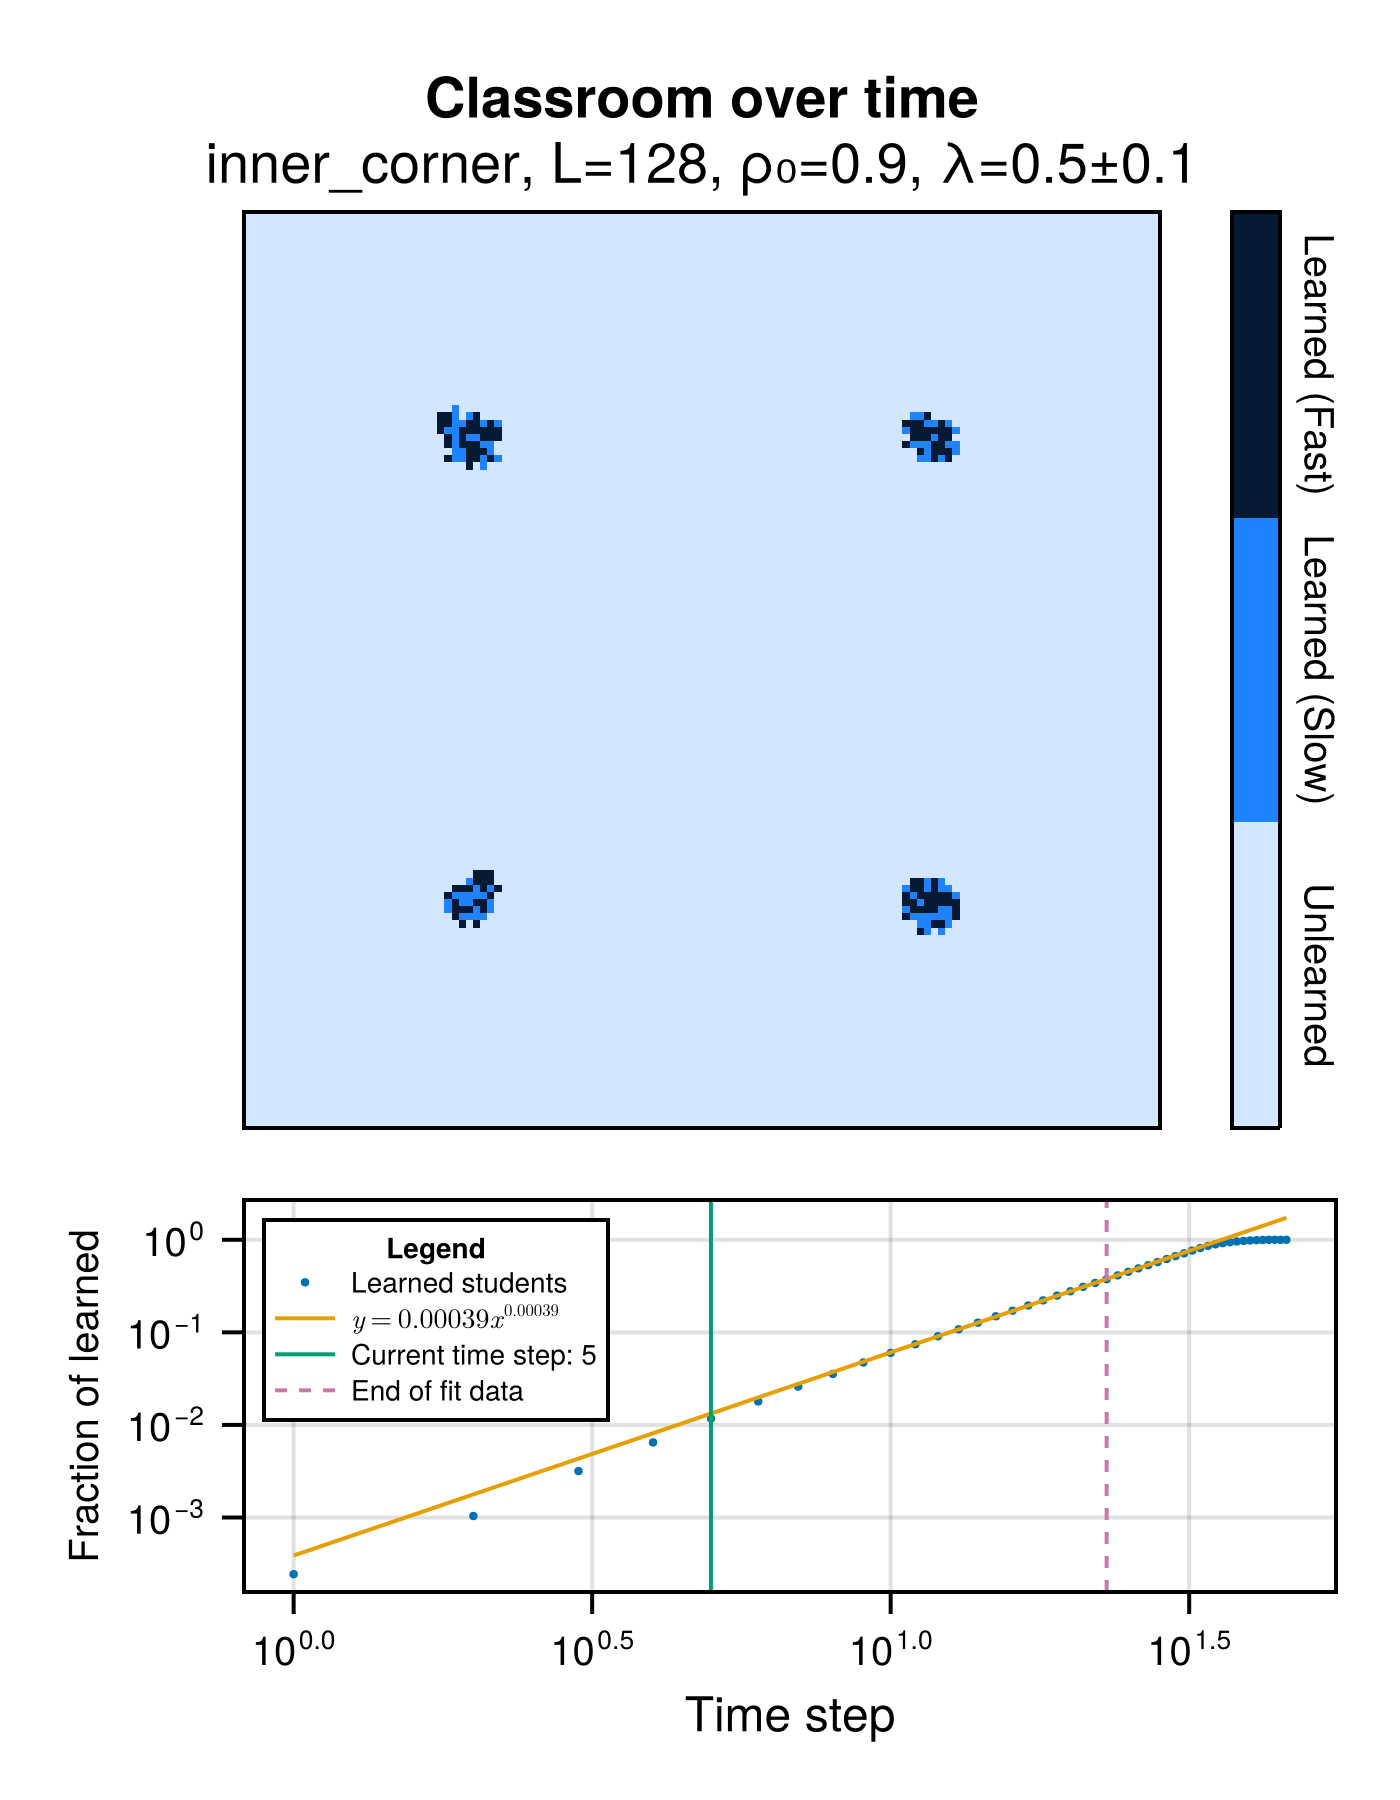
\includegraphics[width=0.49\textwidth]{figures/2D-BPCAIH-analysis/class evolutions/high rho/2DBPCAIH-inner_corner-128-0.9-0.5-0.1-trial_3-5.png}}
    \subfigure[$t=16$]{\label{fig:2DBPCAIH class evolution high rho 16}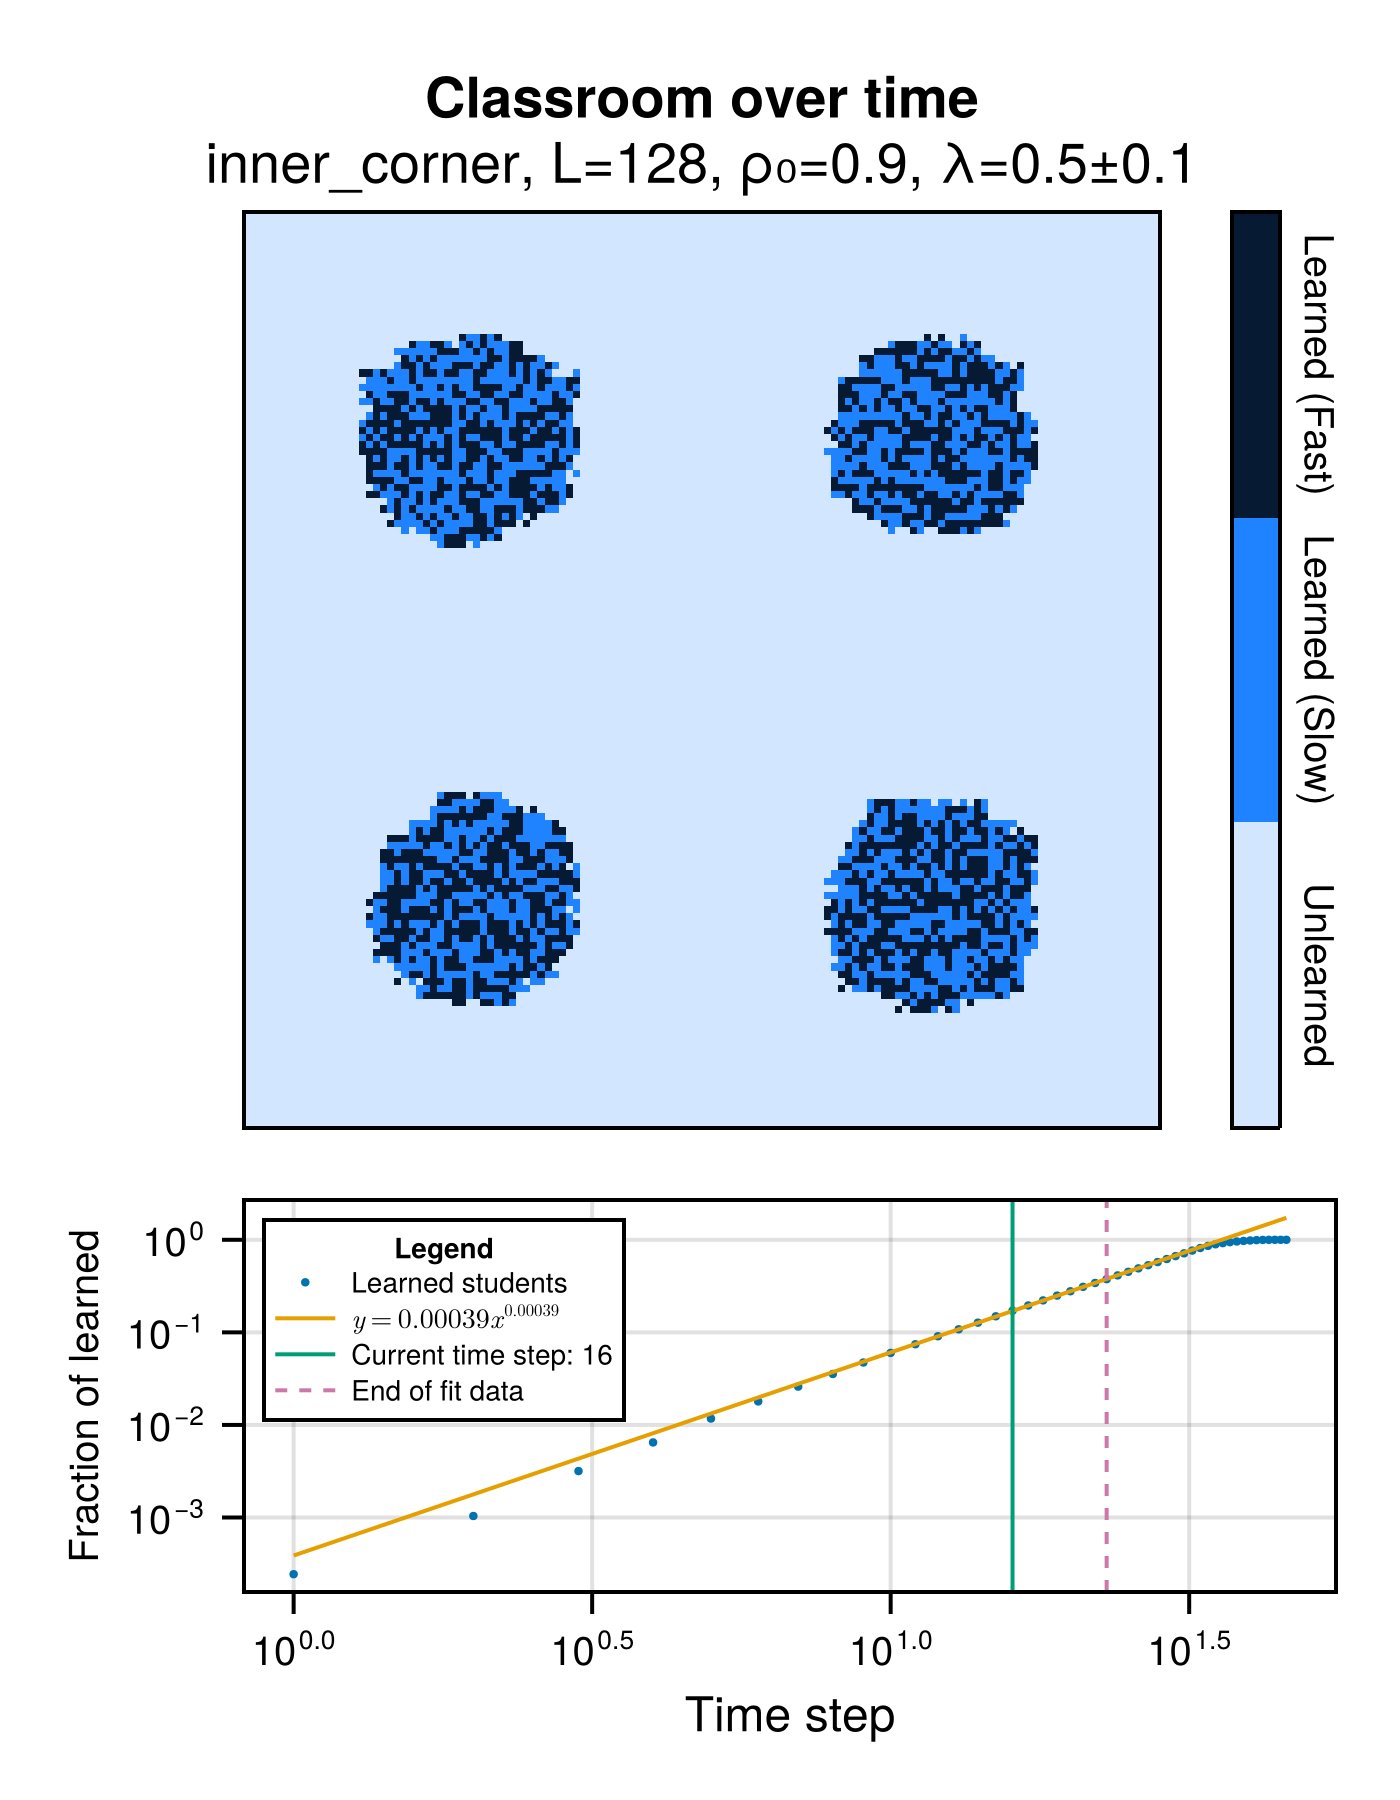
\includegraphics[width=0.49\textwidth]{figures/2D-BPCAIH-analysis/class evolutions/high rho/2DBPCAIH-inner_corner-128-0.9-0.5-0.1-trial_3-16.png}}
    \subfigure[$t=30$]{\label{fig:2DBPCAIH class evolution high rho 30}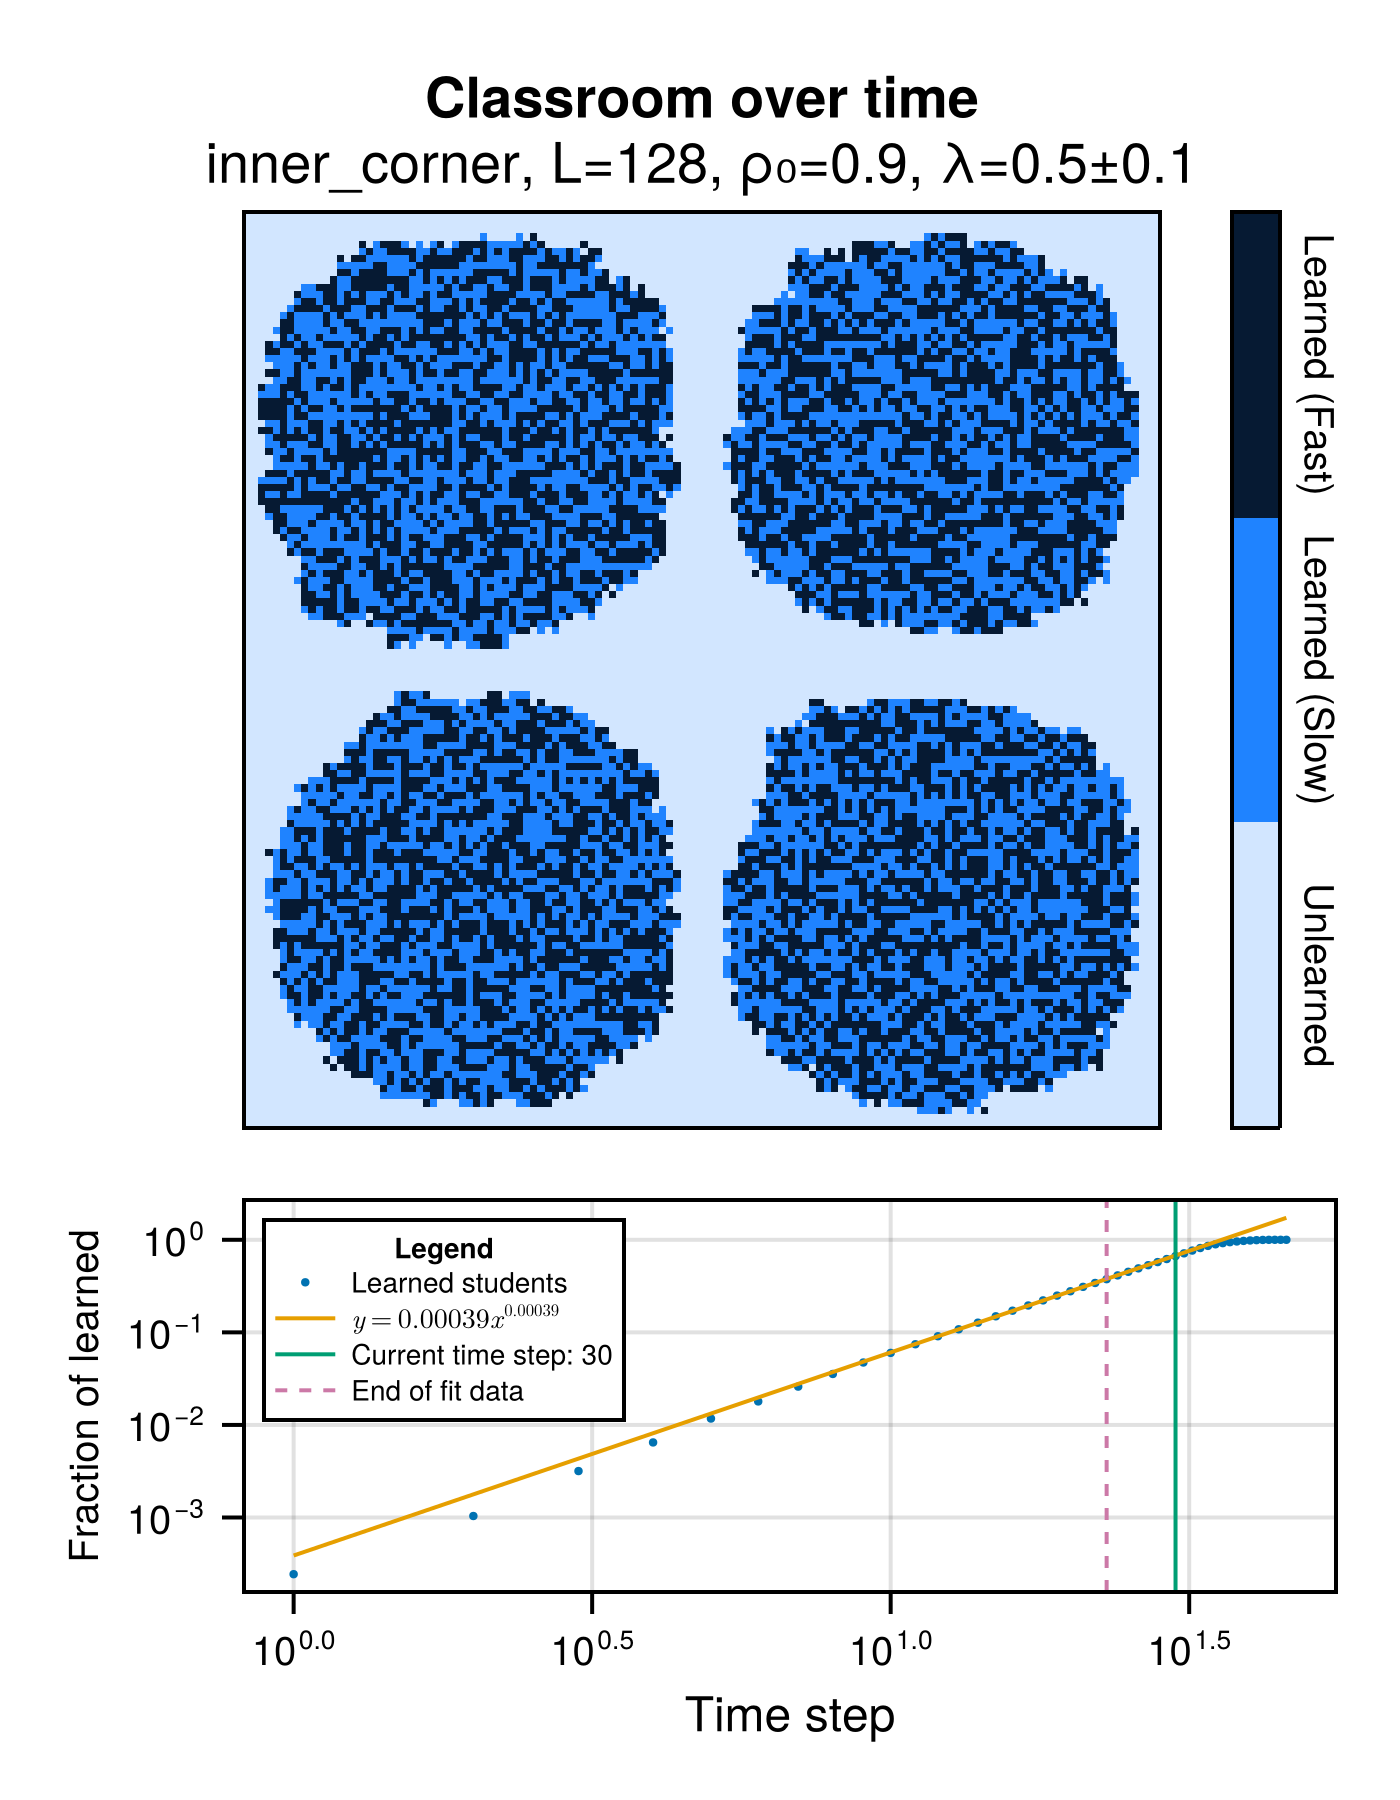
\includegraphics[width=0.49\textwidth]{figures/2D-BPCAIH-analysis/class evolutions/high rho/2DBPCAIH-inner_corner-128-0.9-0.5-0.1-trial_3-30.png}}
    \subfigure[$t=36$]{\label{fig:2DBPCAIH class evolution high rho 36}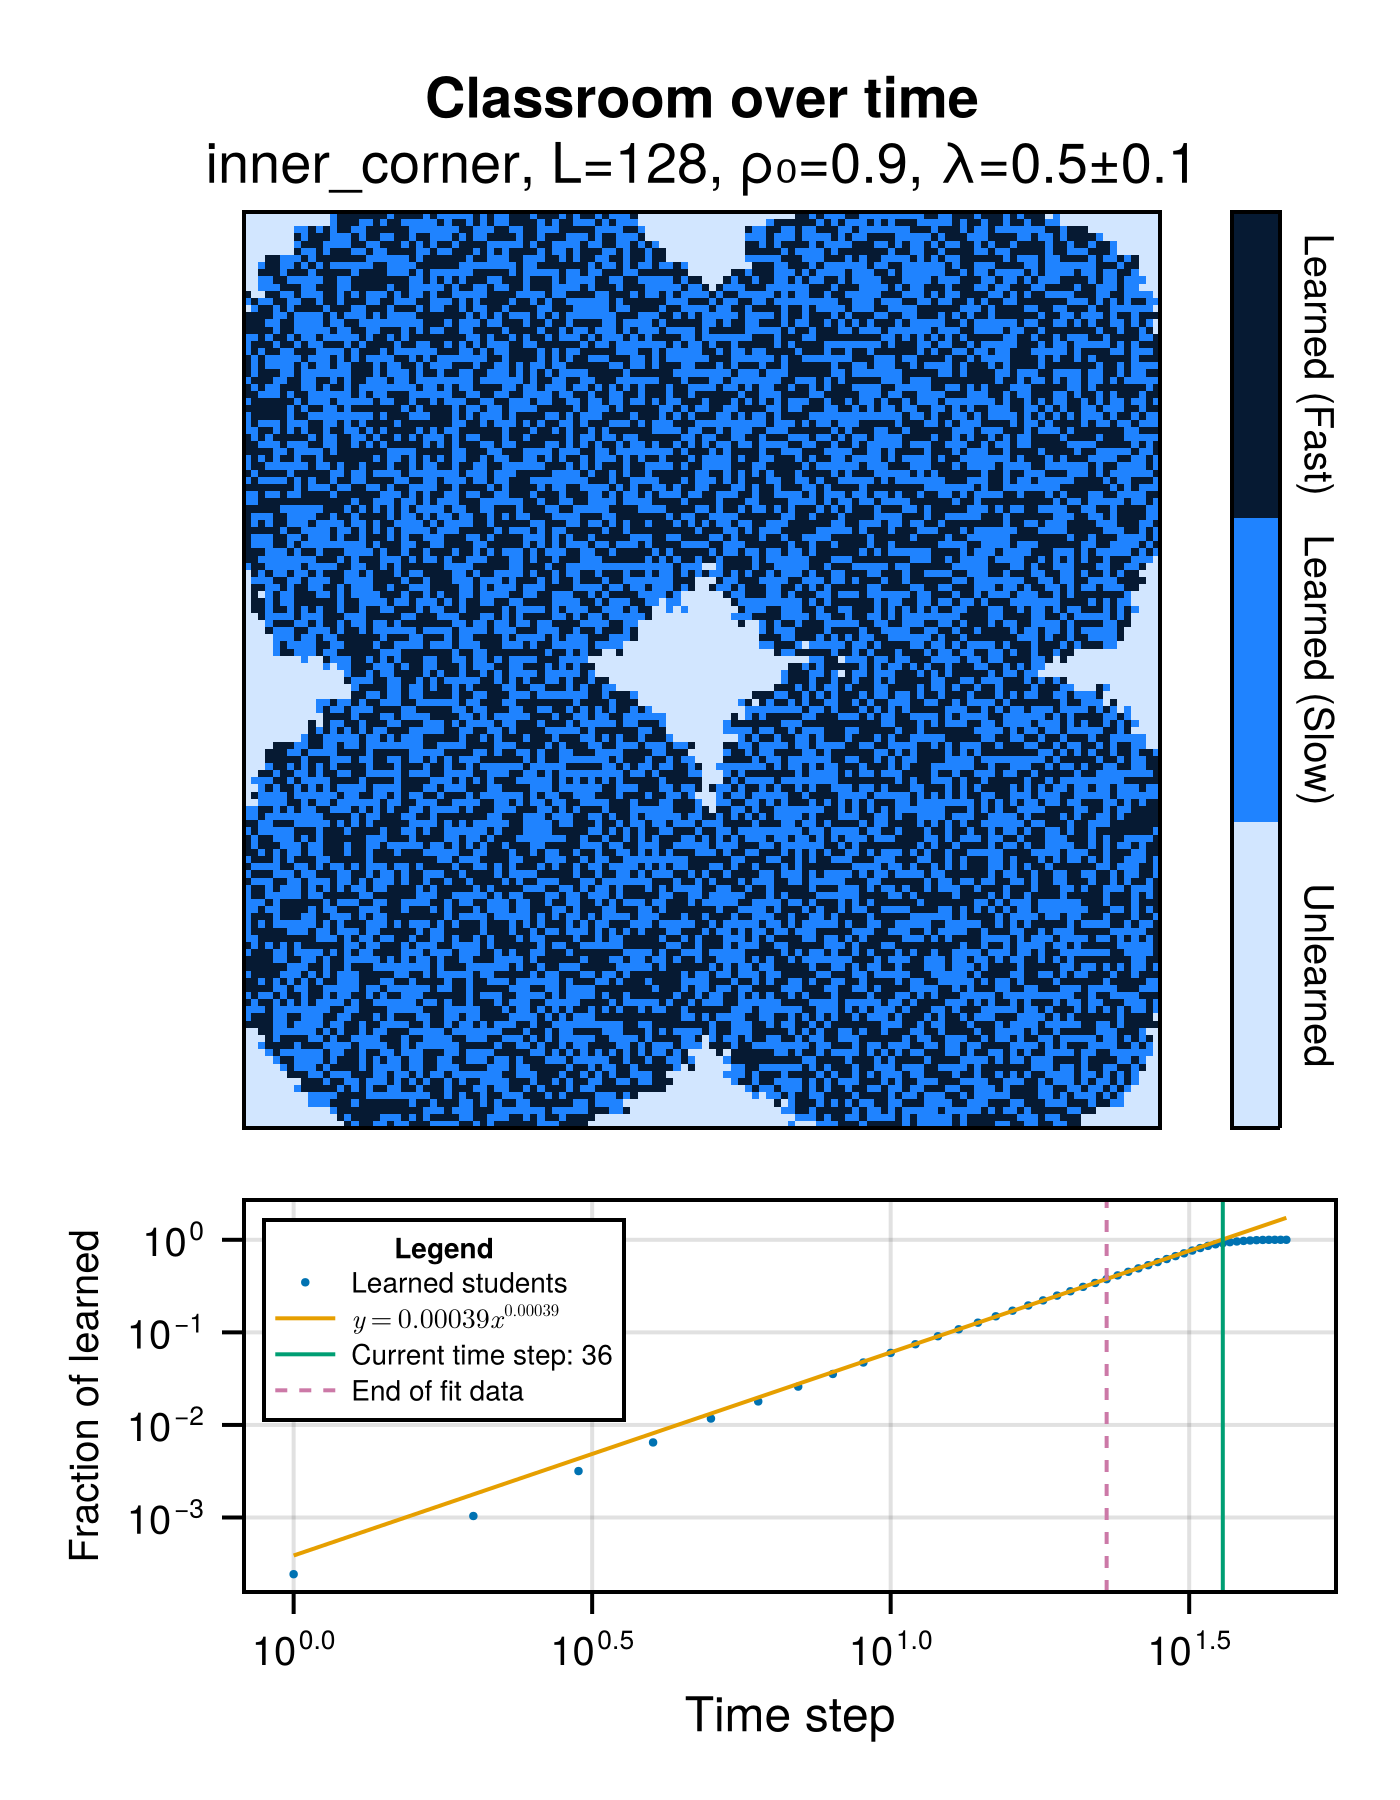
\includegraphics[width=0.49\textwidth]{figures/2D-BPCAIH-analysis/class evolutions/high rho/2DBPCAIH-inner_corner-128-0.9-0.5-0.1-trial_3-36.png}}   
    \caption{Sample classroom evolutions for the inner corner configuration with $L=128$ at different times $t$ for positional learning rate $\rho_0=0.9$, $\delta\lambda = 0.1$.}
    \label{fig:2DBPCAIH sample class evolution high rho}
 \end{figure}

 \begin{figure}[htbp!]
    \centering
    \subfigure[$t=5$]{\label{fig:2DBPCAIH class evolution high rho high delta 5}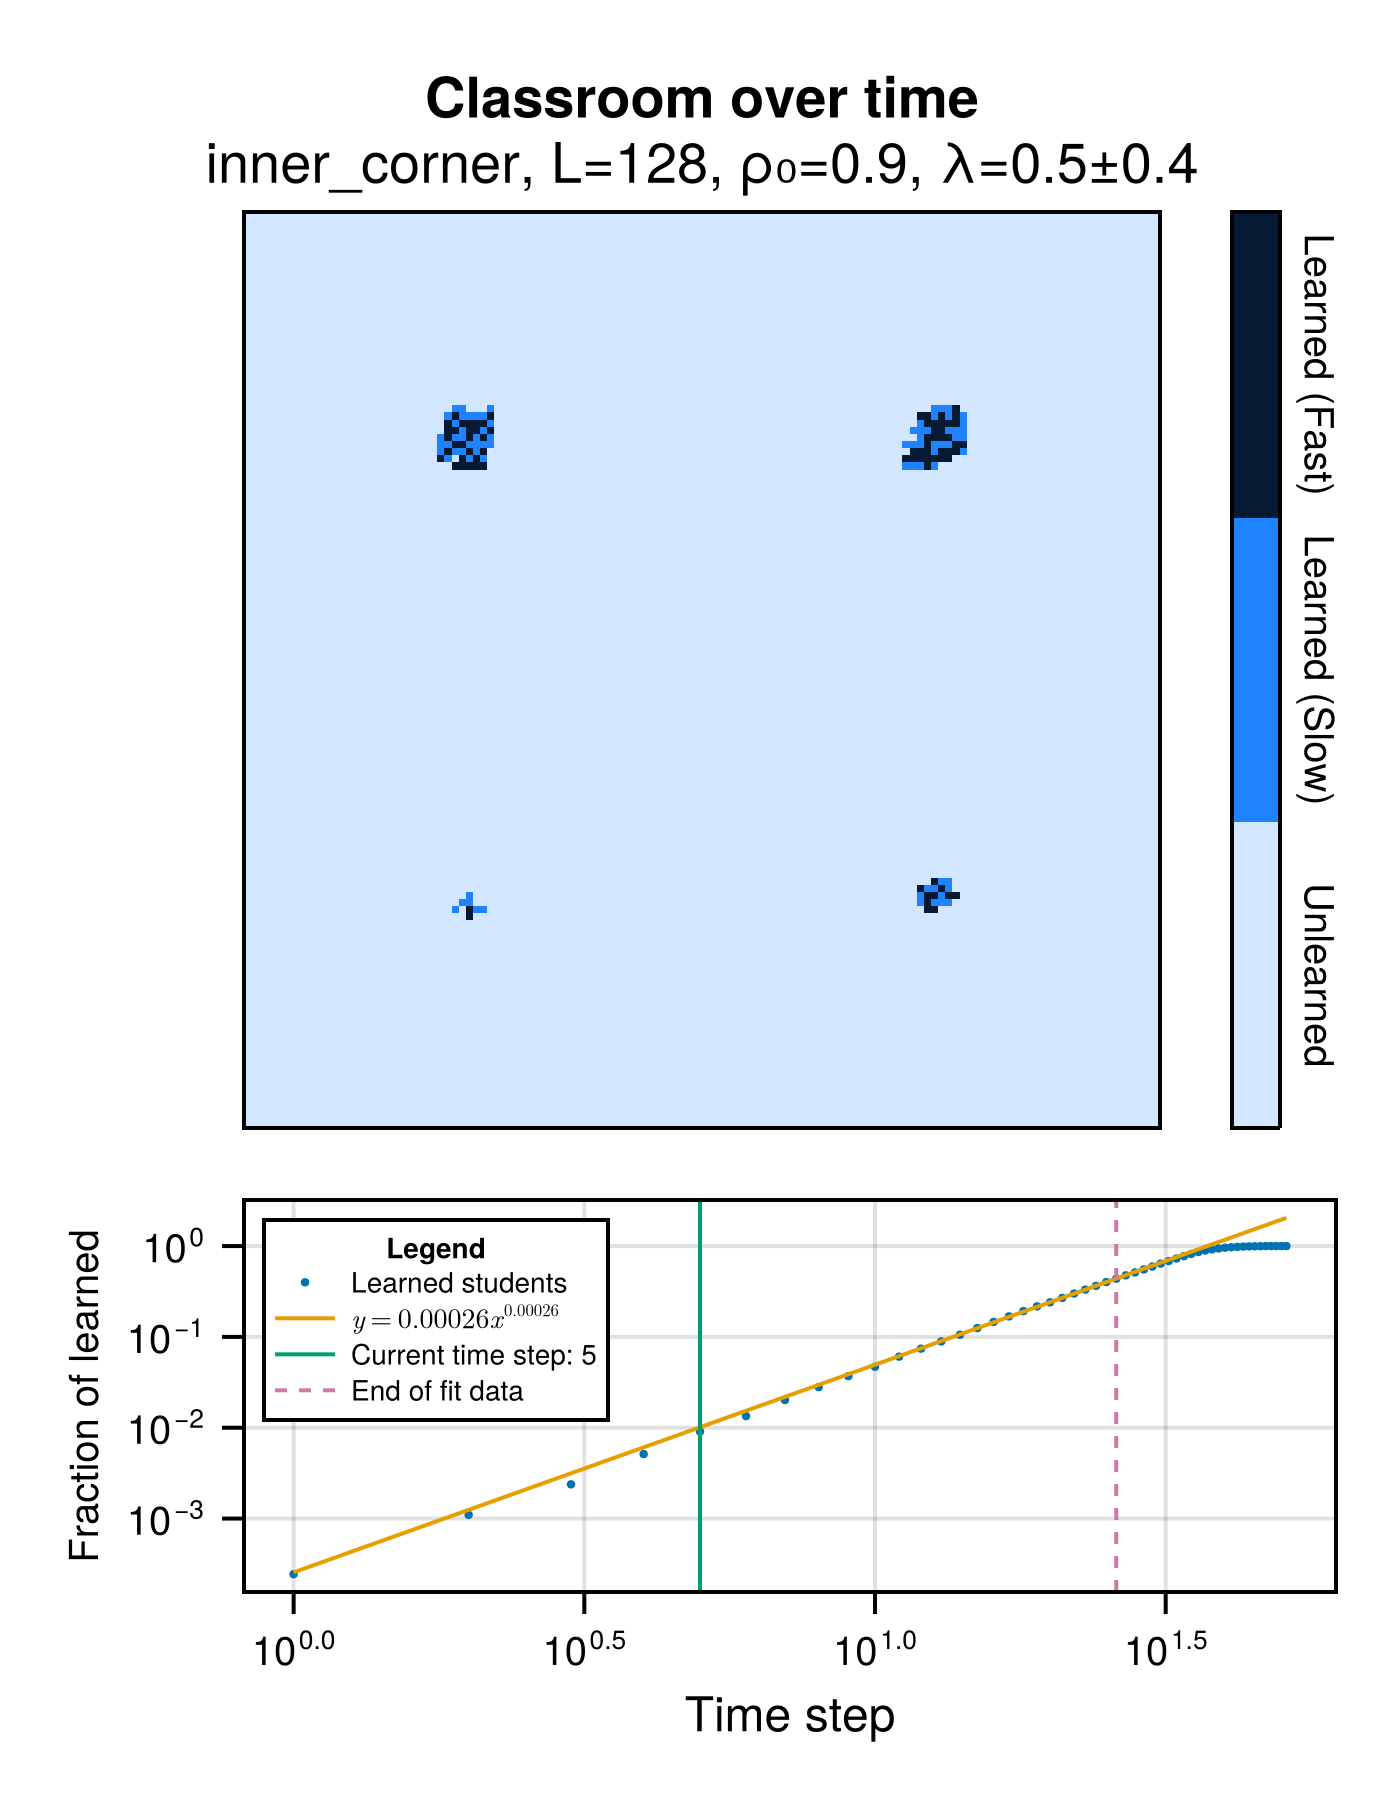
\includegraphics[width=0.49\textwidth]{figures/2D-BPCAIH-analysis/class evolutions/high rho high delta/2DBPCAIH-inner_corner-128-0.9-0.5-0.4-trial_3-5.png}}
    \subfigure[$t=13$]{\label{fig:2DBPCAIH class evolution high rho high delta 13}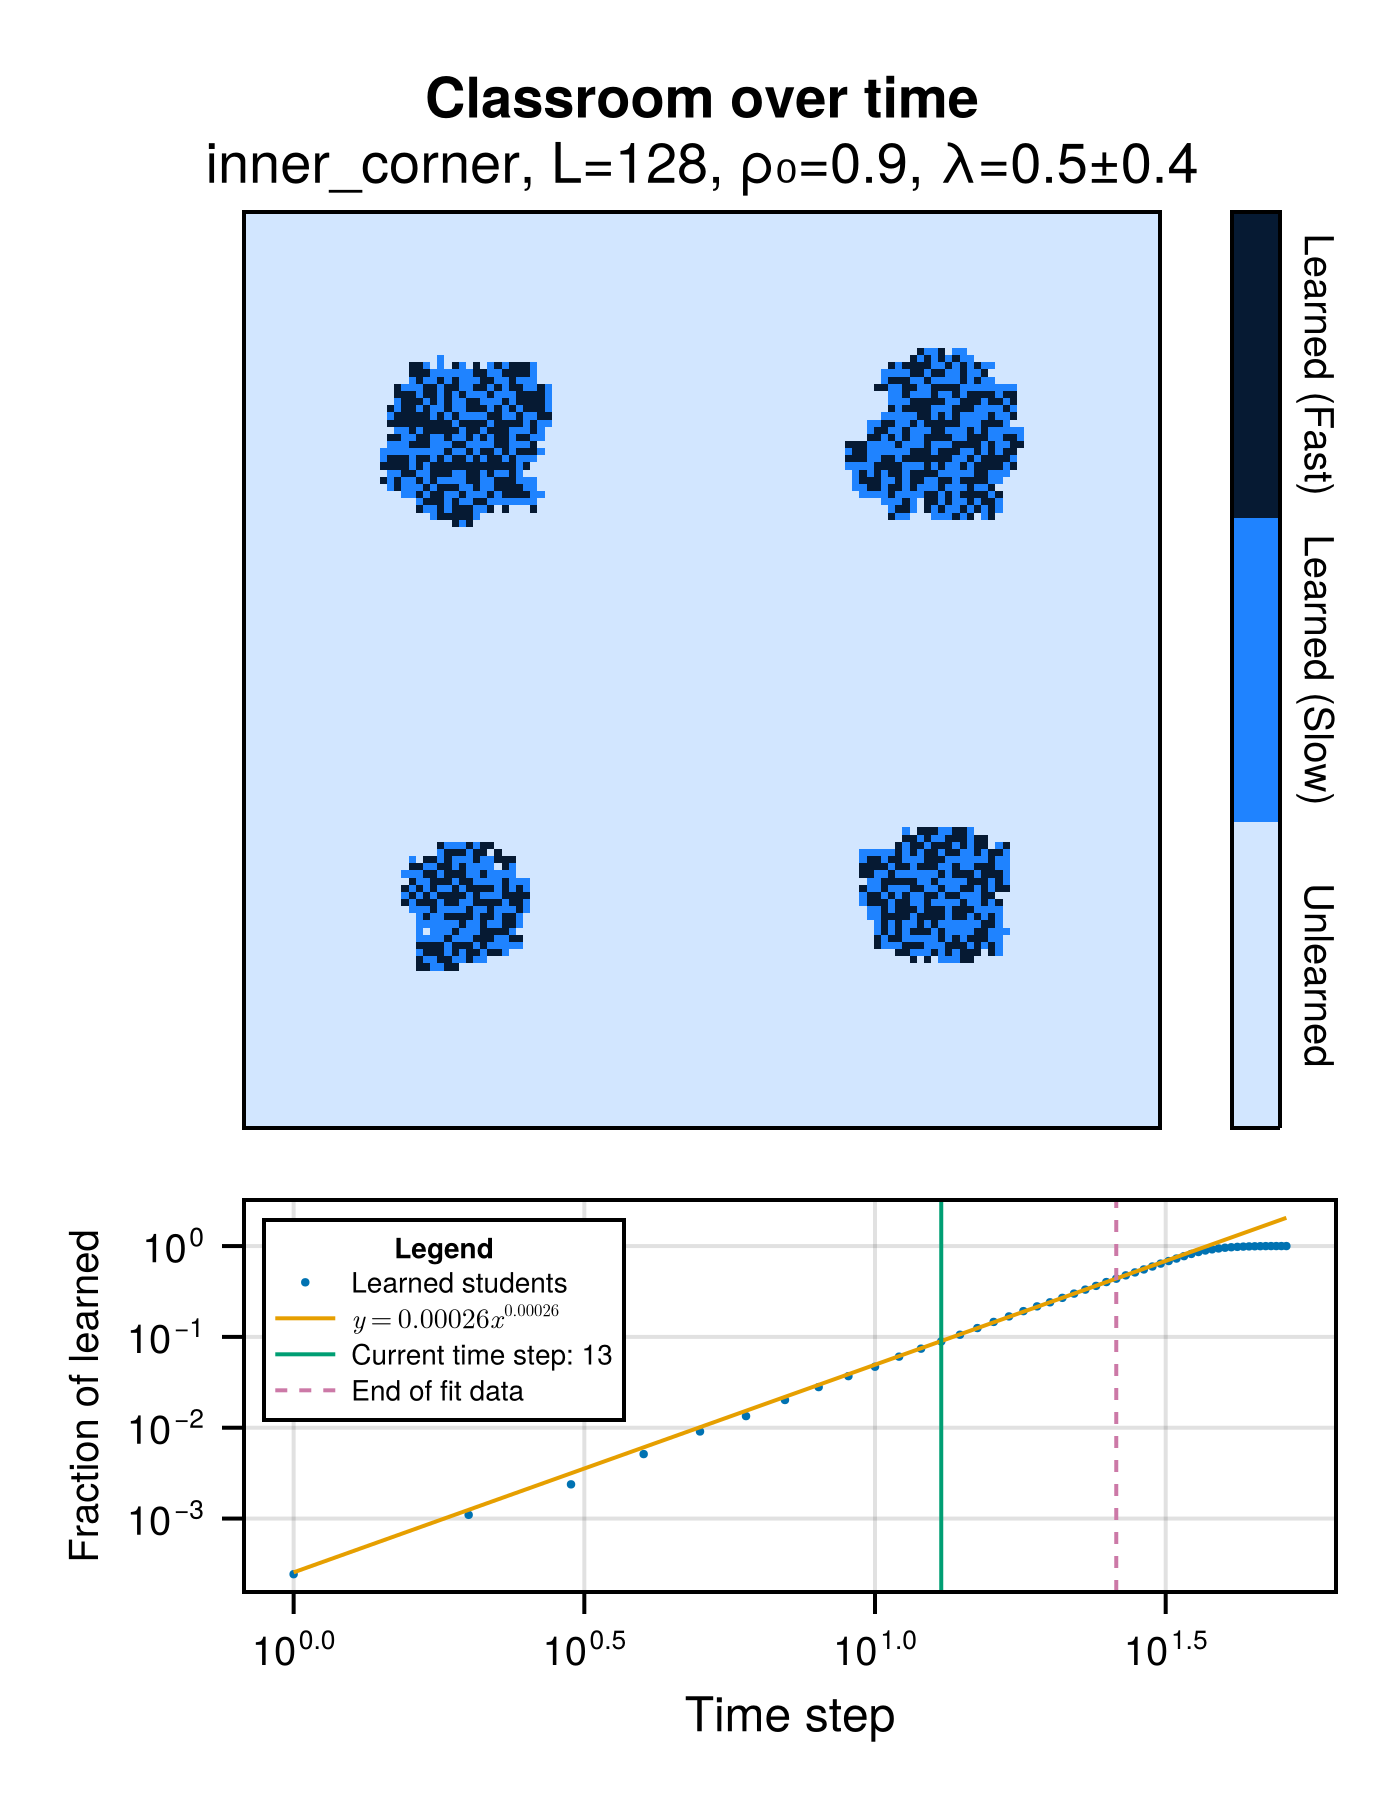
\includegraphics[width=0.49\textwidth]{figures/2D-BPCAIH-analysis/class evolutions/high rho high delta/2DBPCAIH-inner_corner-128-0.9-0.5-0.4-trial_3-13.png}}
    \subfigure[$t=19$]{\label{fig:2DBPCAIH class evolution high rho high delta 19}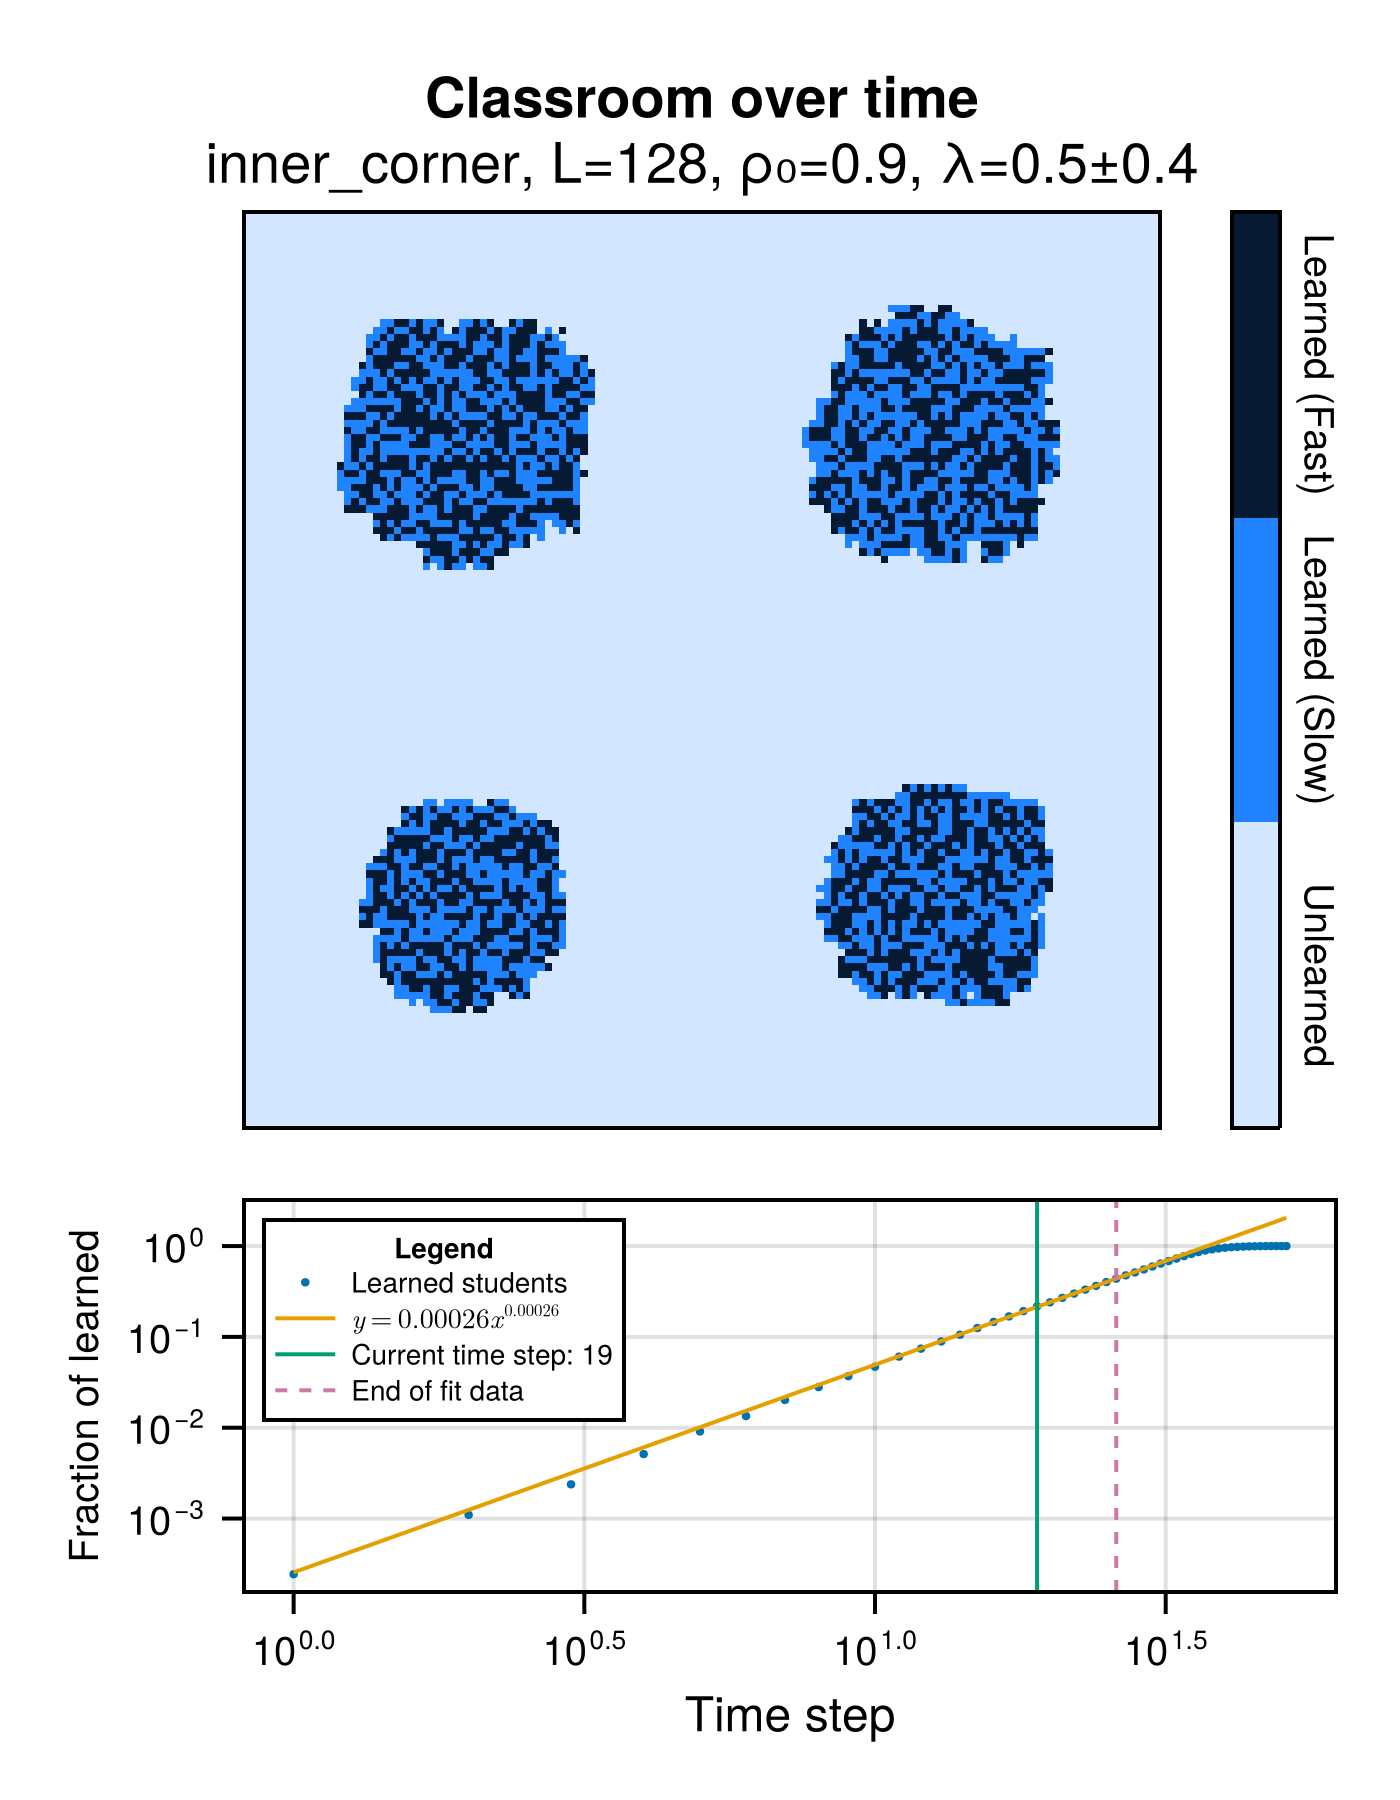
\includegraphics[width=0.49\textwidth]{figures/2D-BPCAIH-analysis/class evolutions/high rho high delta/2DBPCAIH-inner_corner-128-0.9-0.5-0.4-trial_3-19.png}}
    \subfigure[$t=29$]{\label{fig:2DBPCAIH class evolution high rho high delta 29}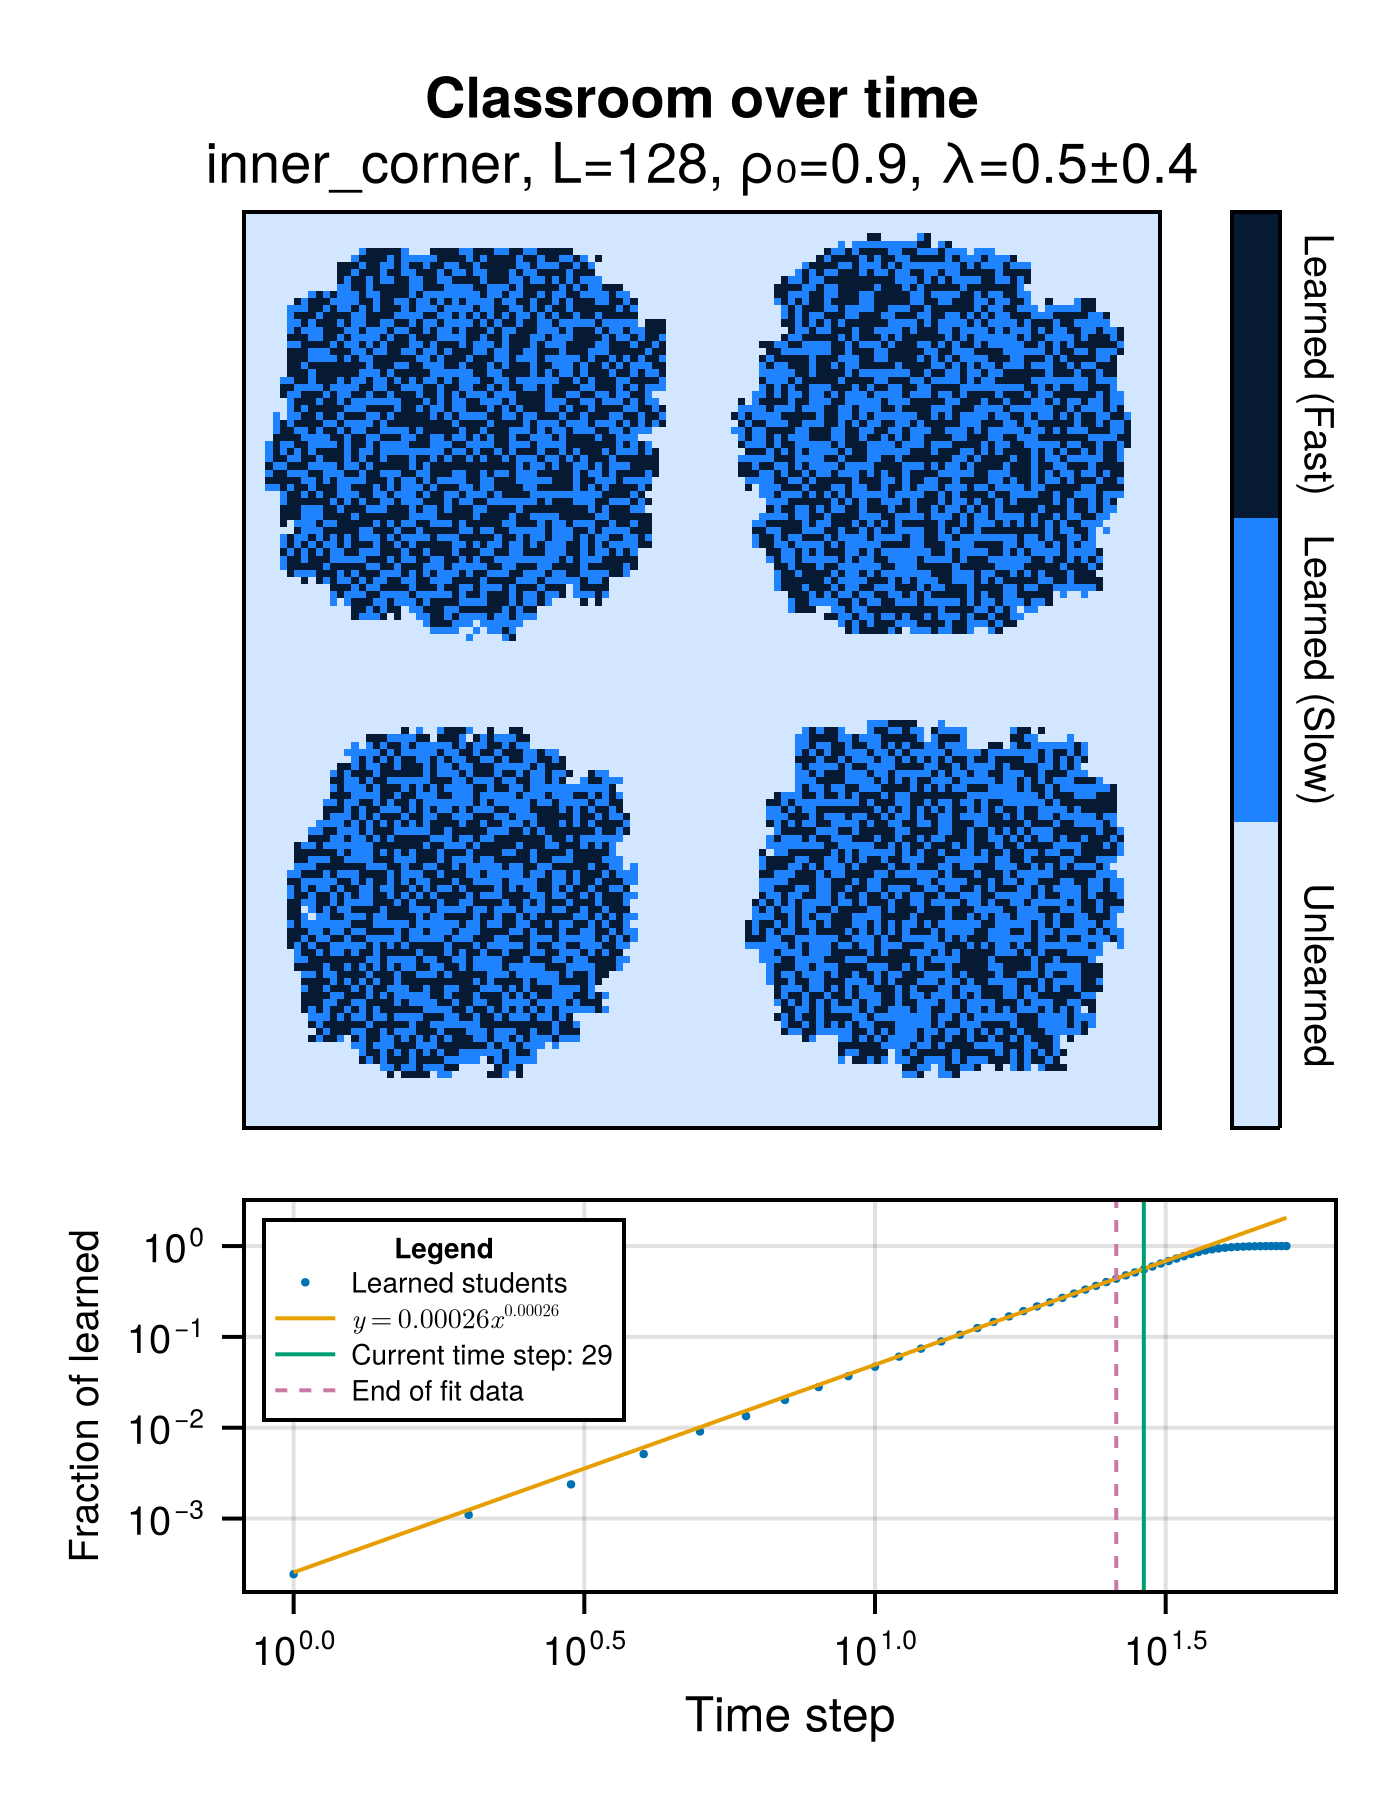
\includegraphics[width=0.49\textwidth]{figures/2D-BPCAIH-analysis/class evolutions/high rho high delta/2DBPCAIH-inner_corner-128-0.9-0.5-0.4-trial_3-29.png}}
    \caption{Sample classroom evolutions for the inner corner configuration with $L=128$ at different times $t$ for positional learning rate $\rho_0=0.9$, $\delta\lambda = 0.4$.}
    \label{fig:2DBPCAIH sample class evolution high rho high delta}
 \end{figure}

\subsection{$m$ vs $\rho$}\label{subsec:BPCAIH m vs rho}

\subsection{$t_{max}$ vs $\rho_0$}\label{subsec:BPCAIH t vs rho}
Figure \ref{fig:2DBPCAIH t-rho plot} shows the time to learn $t_{max}$ is directly affected by the level of heterogeneity $\delta\lambda$. 
This means that the heterogeneity $\delta\lambda$ has a significant effect on the time to learn $t_{max}$, with lower values of $\delta\lambda$ leading to lower time to learn $t_{max}$ for all values of $\rho_0$. 
We also notice that the traditional model is more affected by classroom heterogeneity comapred to PI models.

When aggregating the different results for each class size $L$, as shown in Figure \ref{fig:2DBPCAIH t-rho ribbon plot}, it affirms our previous findings that PI models are better for smaller clases and lower values of $\rho_0$.
This stays consistent when comparing the performance of a similar classroom size $L$ and heterogeneity $\delta\lambda$ using the traditional model.
However, the comparison is not as clear when comparing between different levels of heterogeneity $\delta\lambda$.
When $L\geq64$, the PI models can perform better than the traditional model depending on the heterogeneity $\delta\lambda$, even with the same positional learning factor $\rho_0$.

\begin{figure}[htbp!]
    \centering
    \subfigure[Outer corner $L=48$]{\label{fig:2DBPCAIH t-rho plot OC48}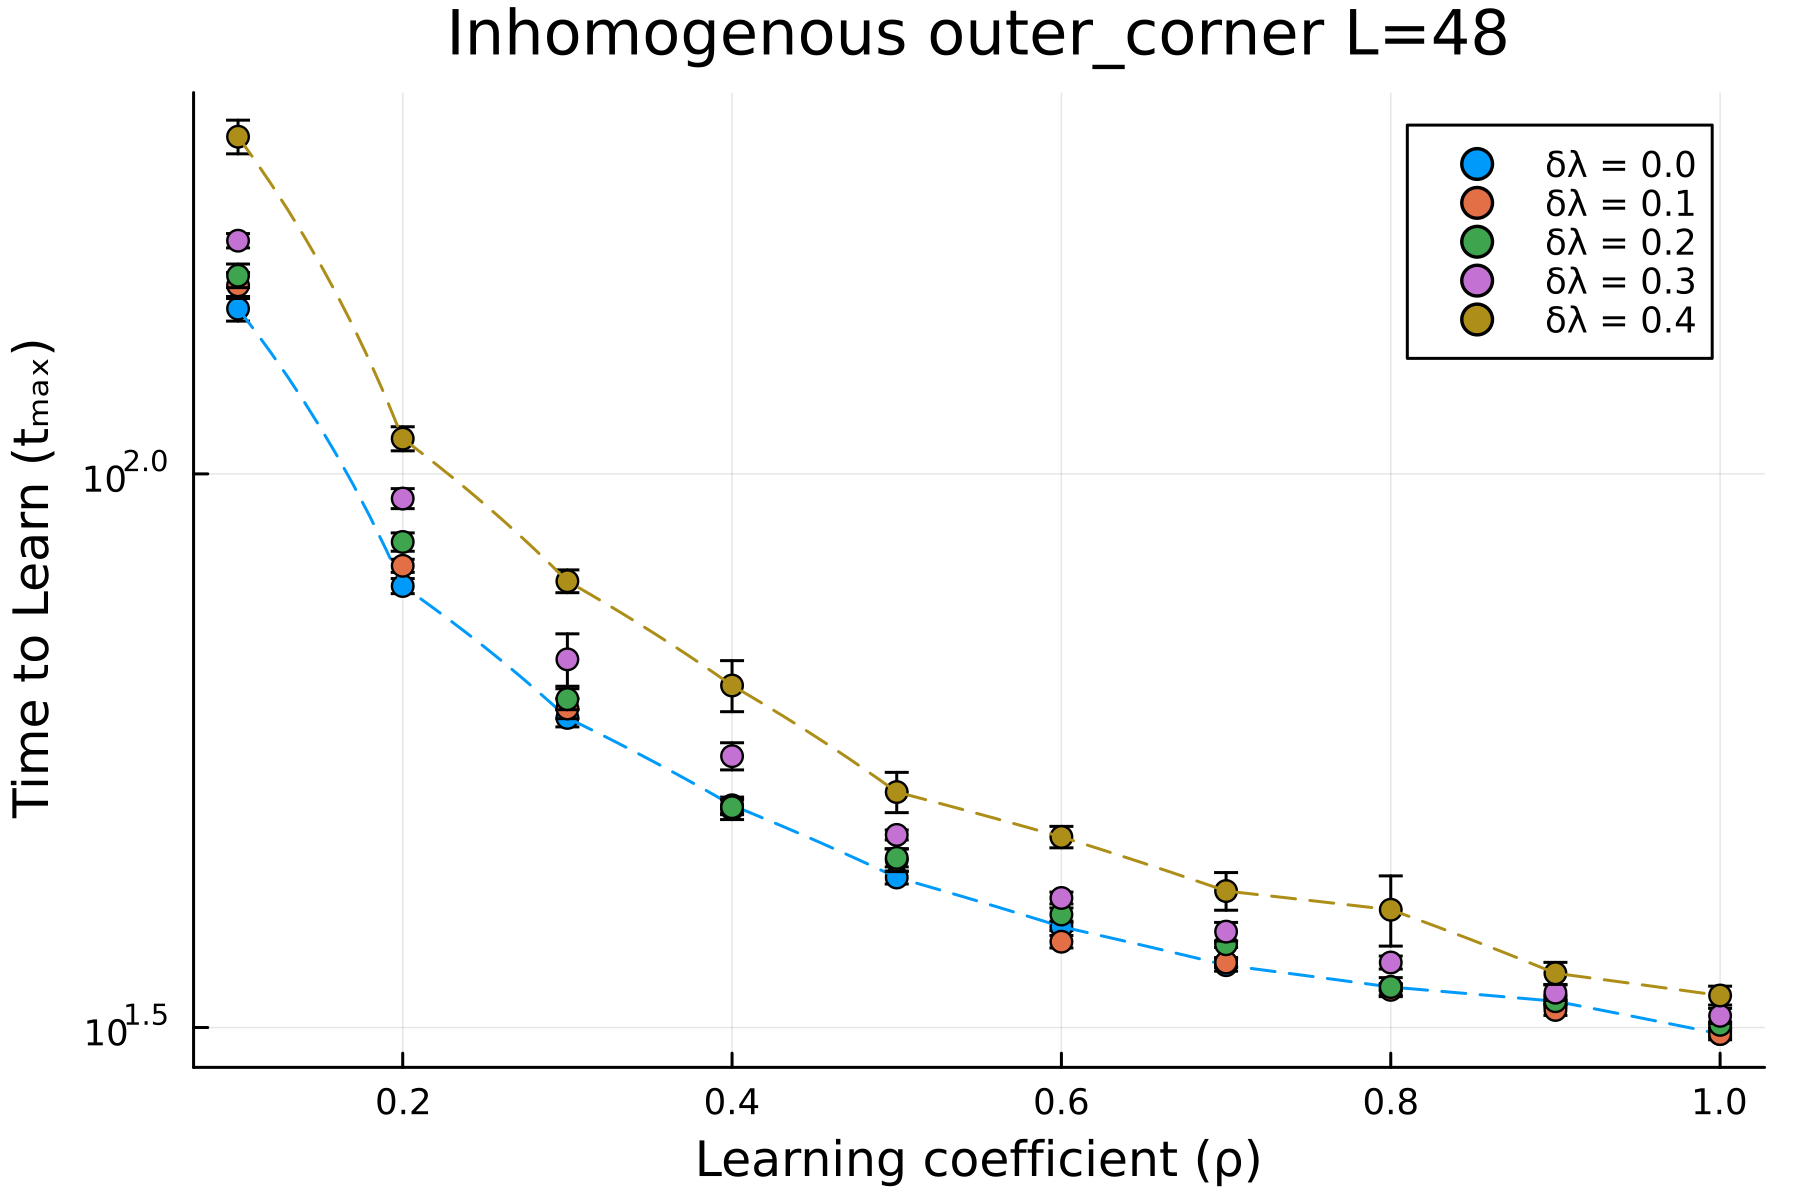
\includegraphics[width=0.49\textwidth]{figures/2D-BPCAIH-analysis/t-plots/t-outer_corner-48.png}}
    \subfigure[Outer corner $L=96$]{\label{fig:2DBPCAIH t-rho plot OC96}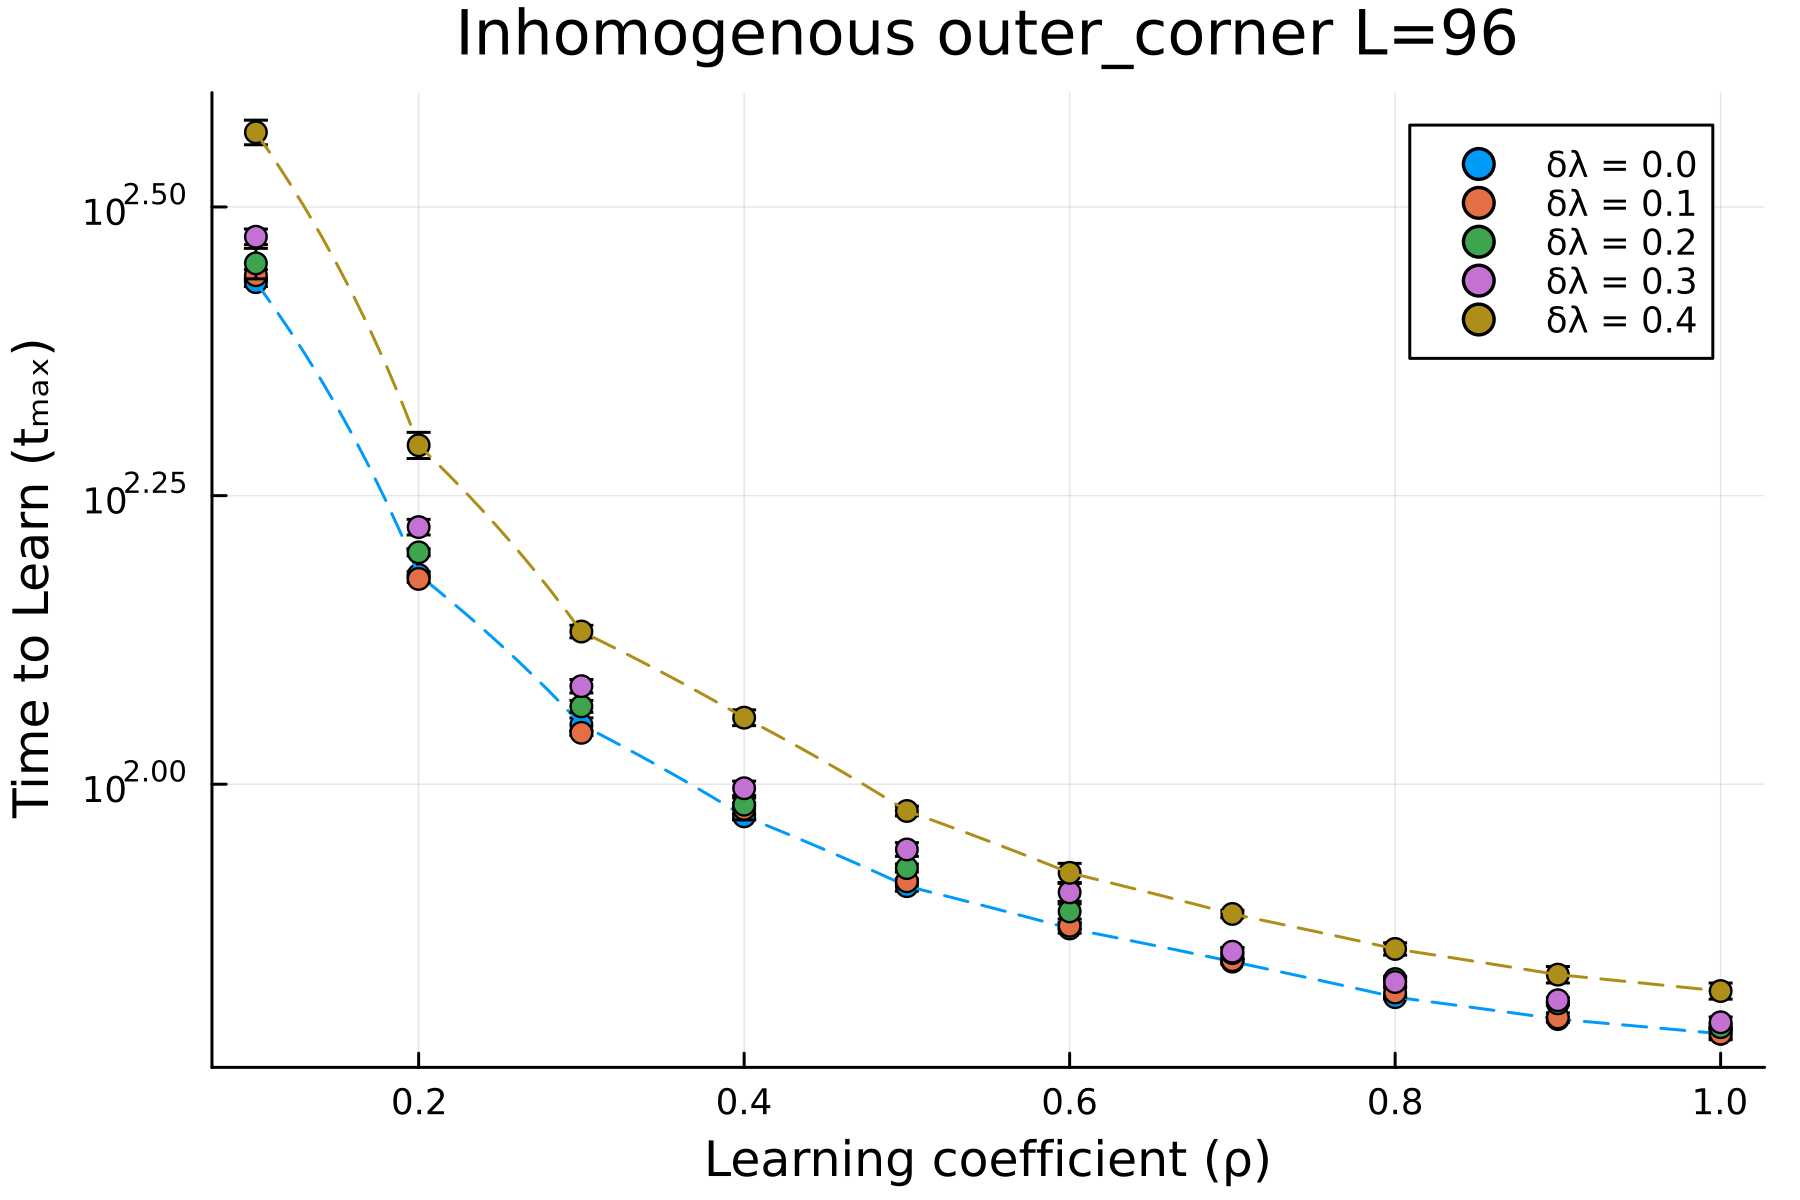
\includegraphics[width=0.49\textwidth]{figures/2D-BPCAIH-analysis/t-plots/t-outer_corner-96.png}}
    \subfigure[Inner corner $L=48$]{\label{fig:2DBPCAIH t-rho plot IC48}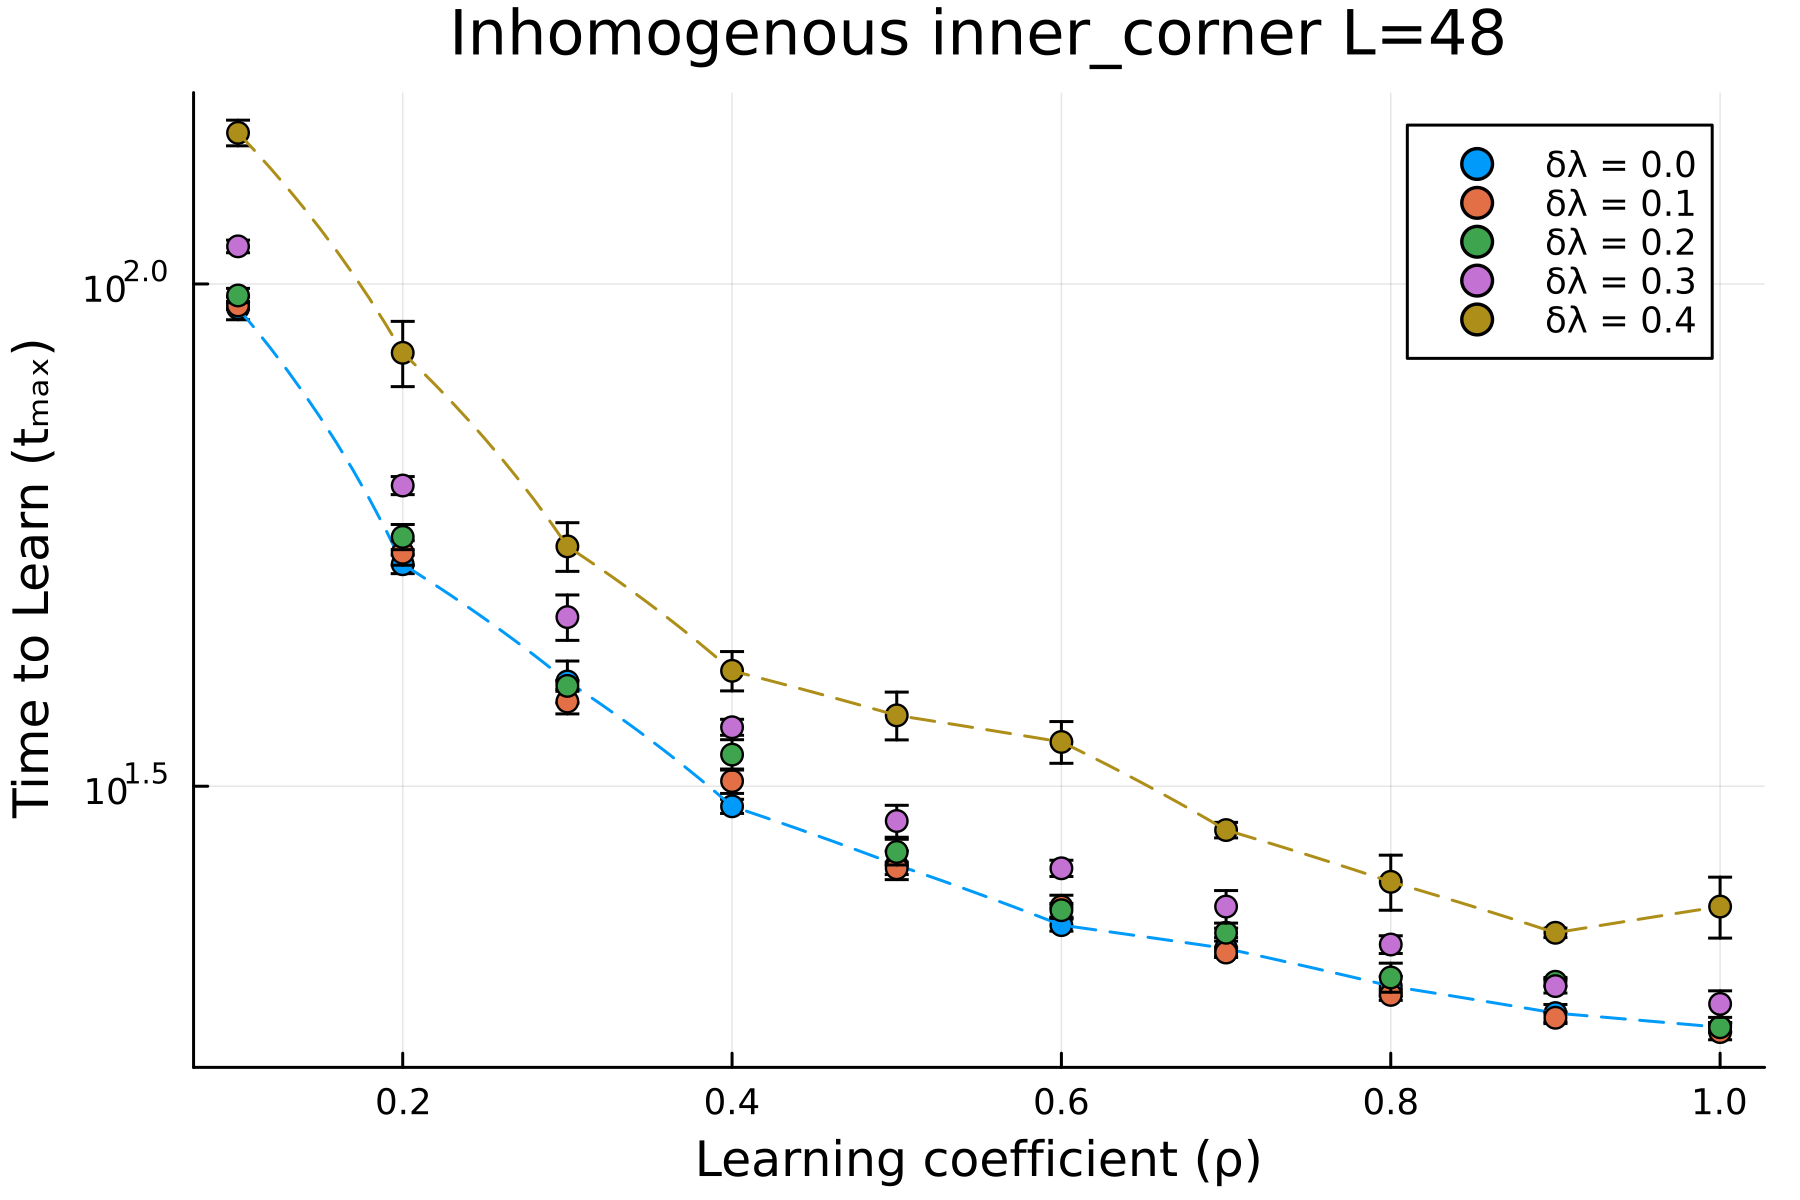
\includegraphics[width=0.49\textwidth]{figures/2D-BPCAIH-analysis/t-plots/t-inner_corner-48.png}}
    \subfigure[Inner corner $L=96$]{\label{fig:2DBPCAIH t-rho plot IC96}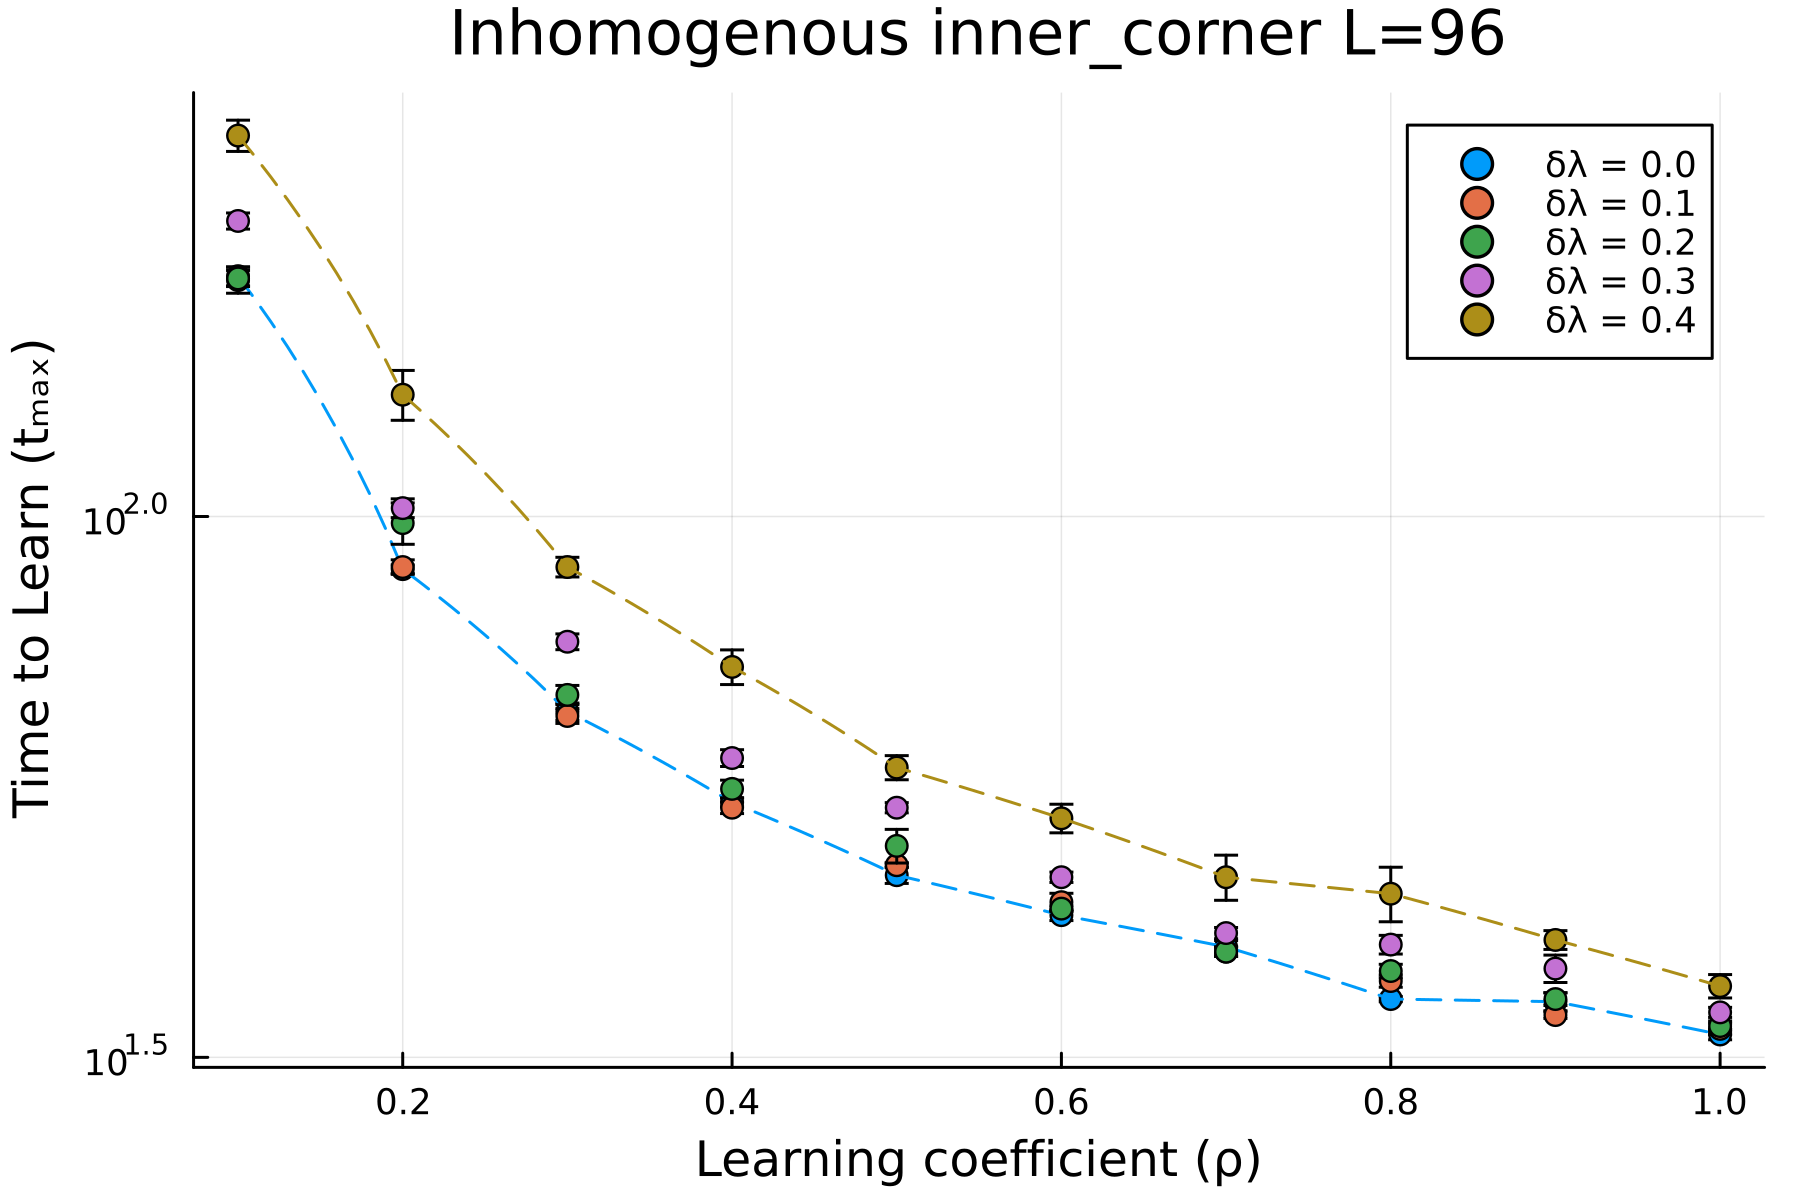
\includegraphics[width=0.49\textwidth]{figures/2D-BPCAIH-analysis/t-plots/t-inner_corner-96.png}}
    \subfigure[Traditional $L=48$]{\label{fig:2DBPCAIH t-rho plot T48}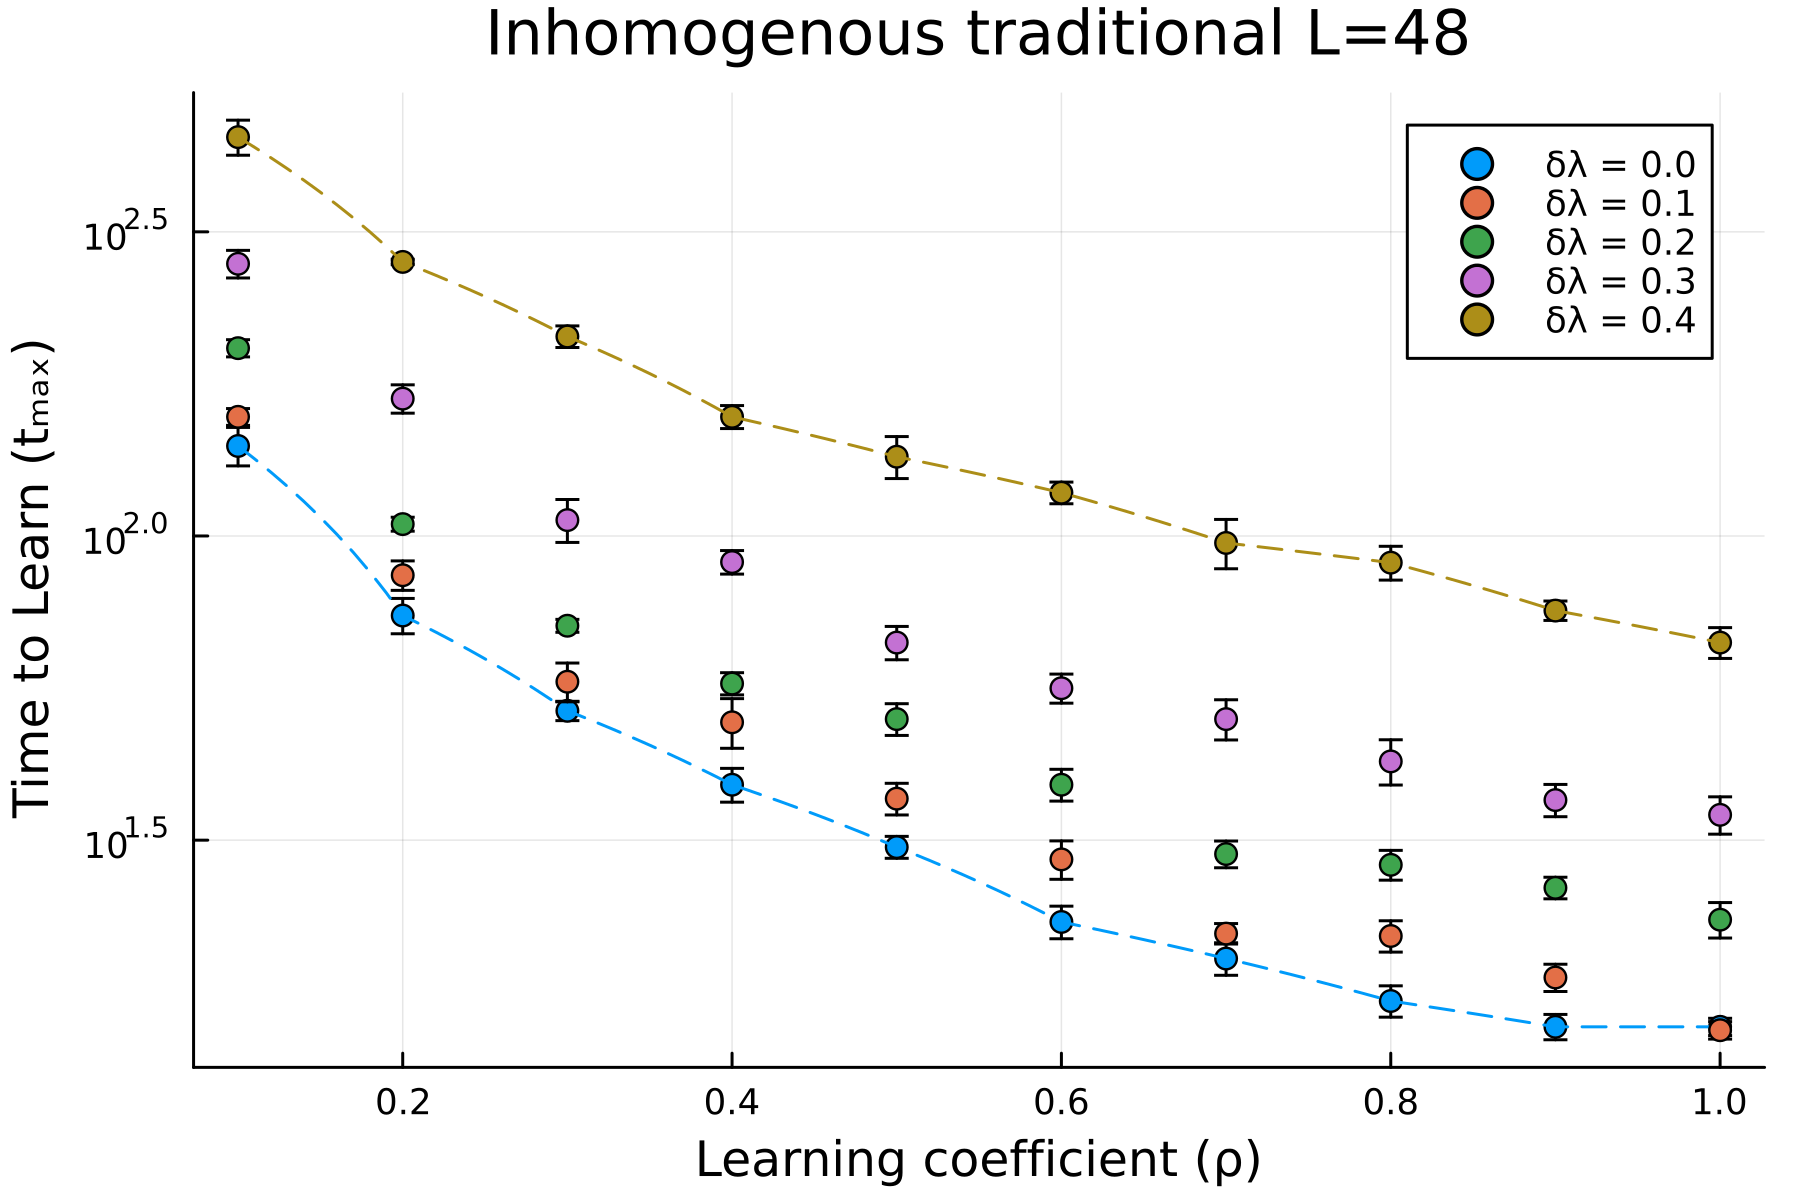
\includegraphics[width=0.49\textwidth]{figures/2D-BPCAIH-analysis/t-plots/t-traditional-48.png}}
    \subfigure[Traditional $L=96$]{\label{fig:2DBPCAIH t-rho plot T96}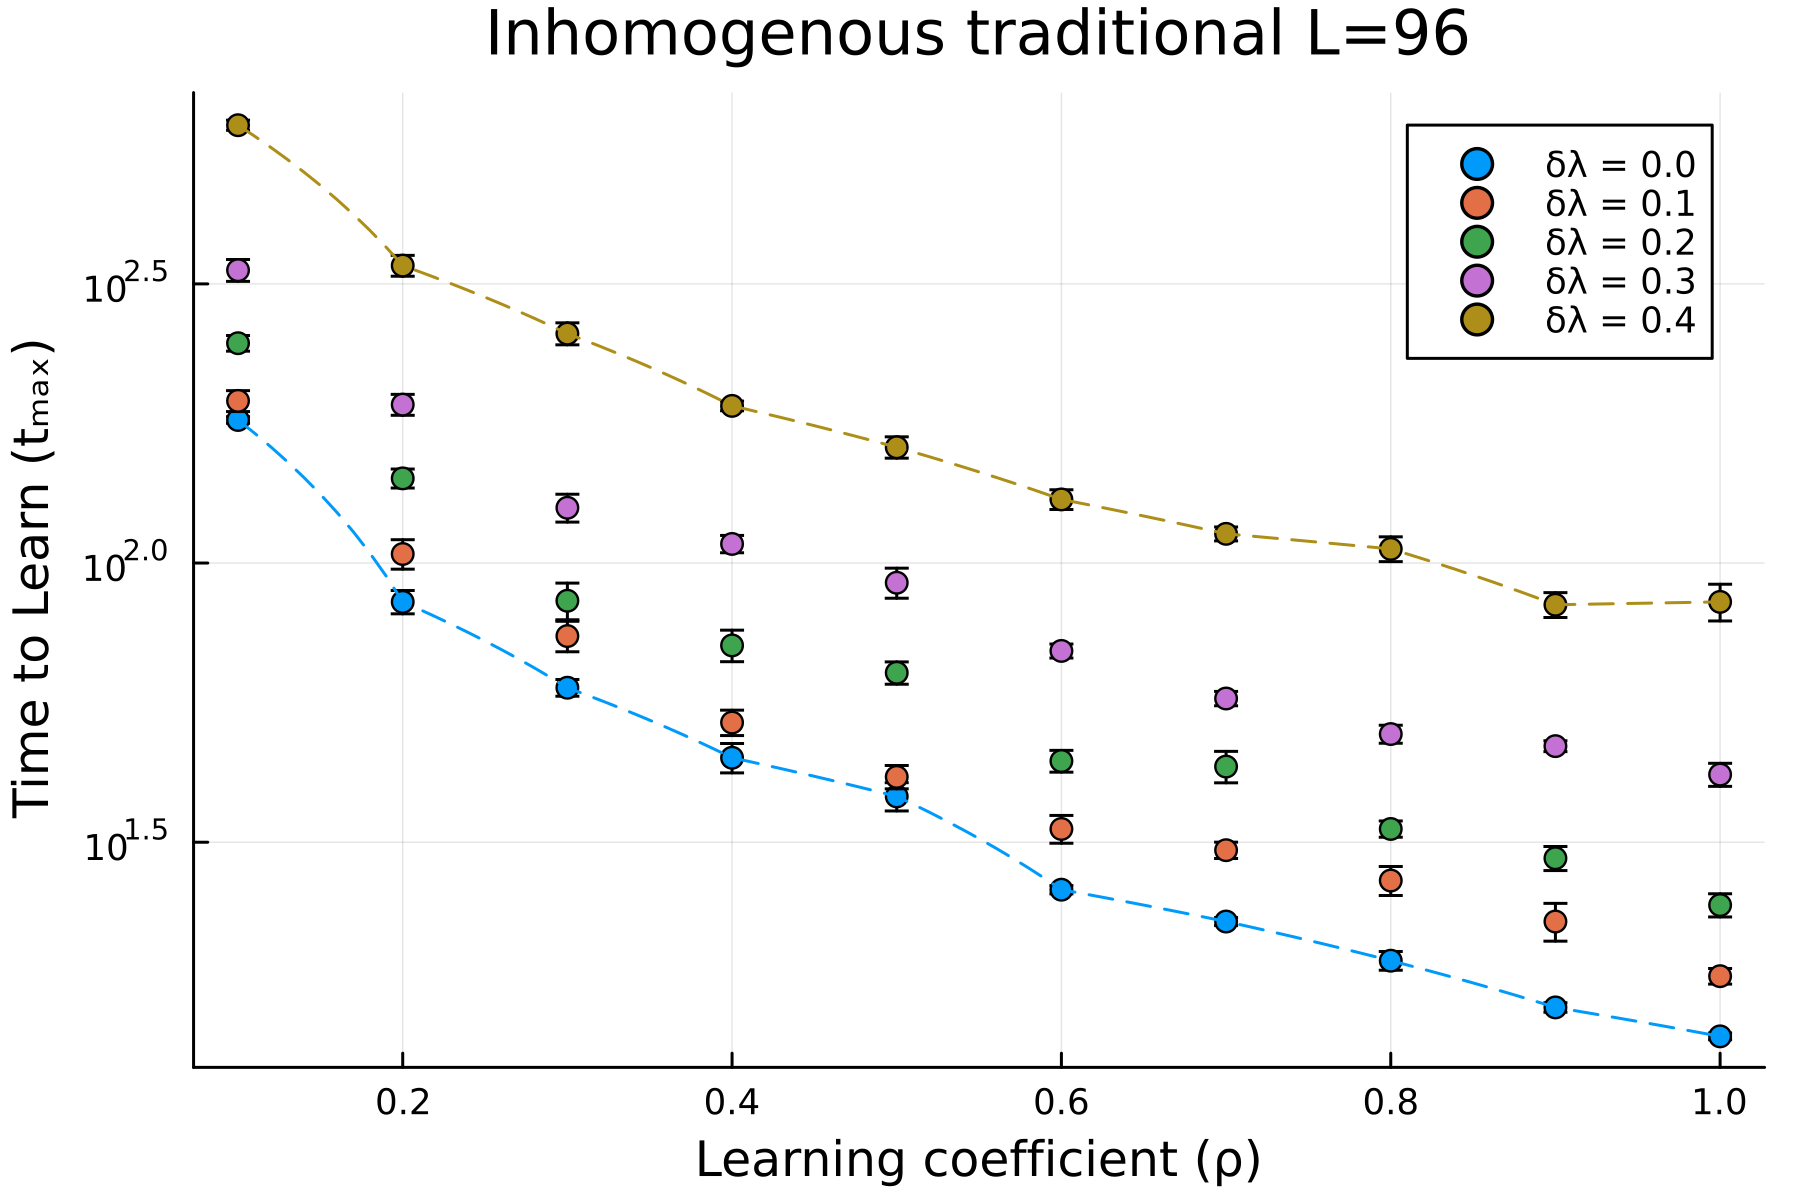
\includegraphics[width=0.49\textwidth]{figures/2D-BPCAIH-analysis/t-plots/t-traditional-96.png}}
    \caption{Time to learn $t_{max}$ as a function of positional learning factor $\rho_0$ for different representative classroom configurations and sizes with varying heterogeneity $\delta\lambda \in \lbrace 0, 0.1, 0.2, 0.3, 0.4 \rbrace$. Lower time to learn $t_{max}$ indicates better performance.}
    \label{fig:2DBPCAIH t-rho plot}
 \end{figure}

 \begin{figure}[htbp!]
    \centering
    \subfigure[$L=32$]{\label{fig:2DBPCAIH t-rho ribbon plot 32}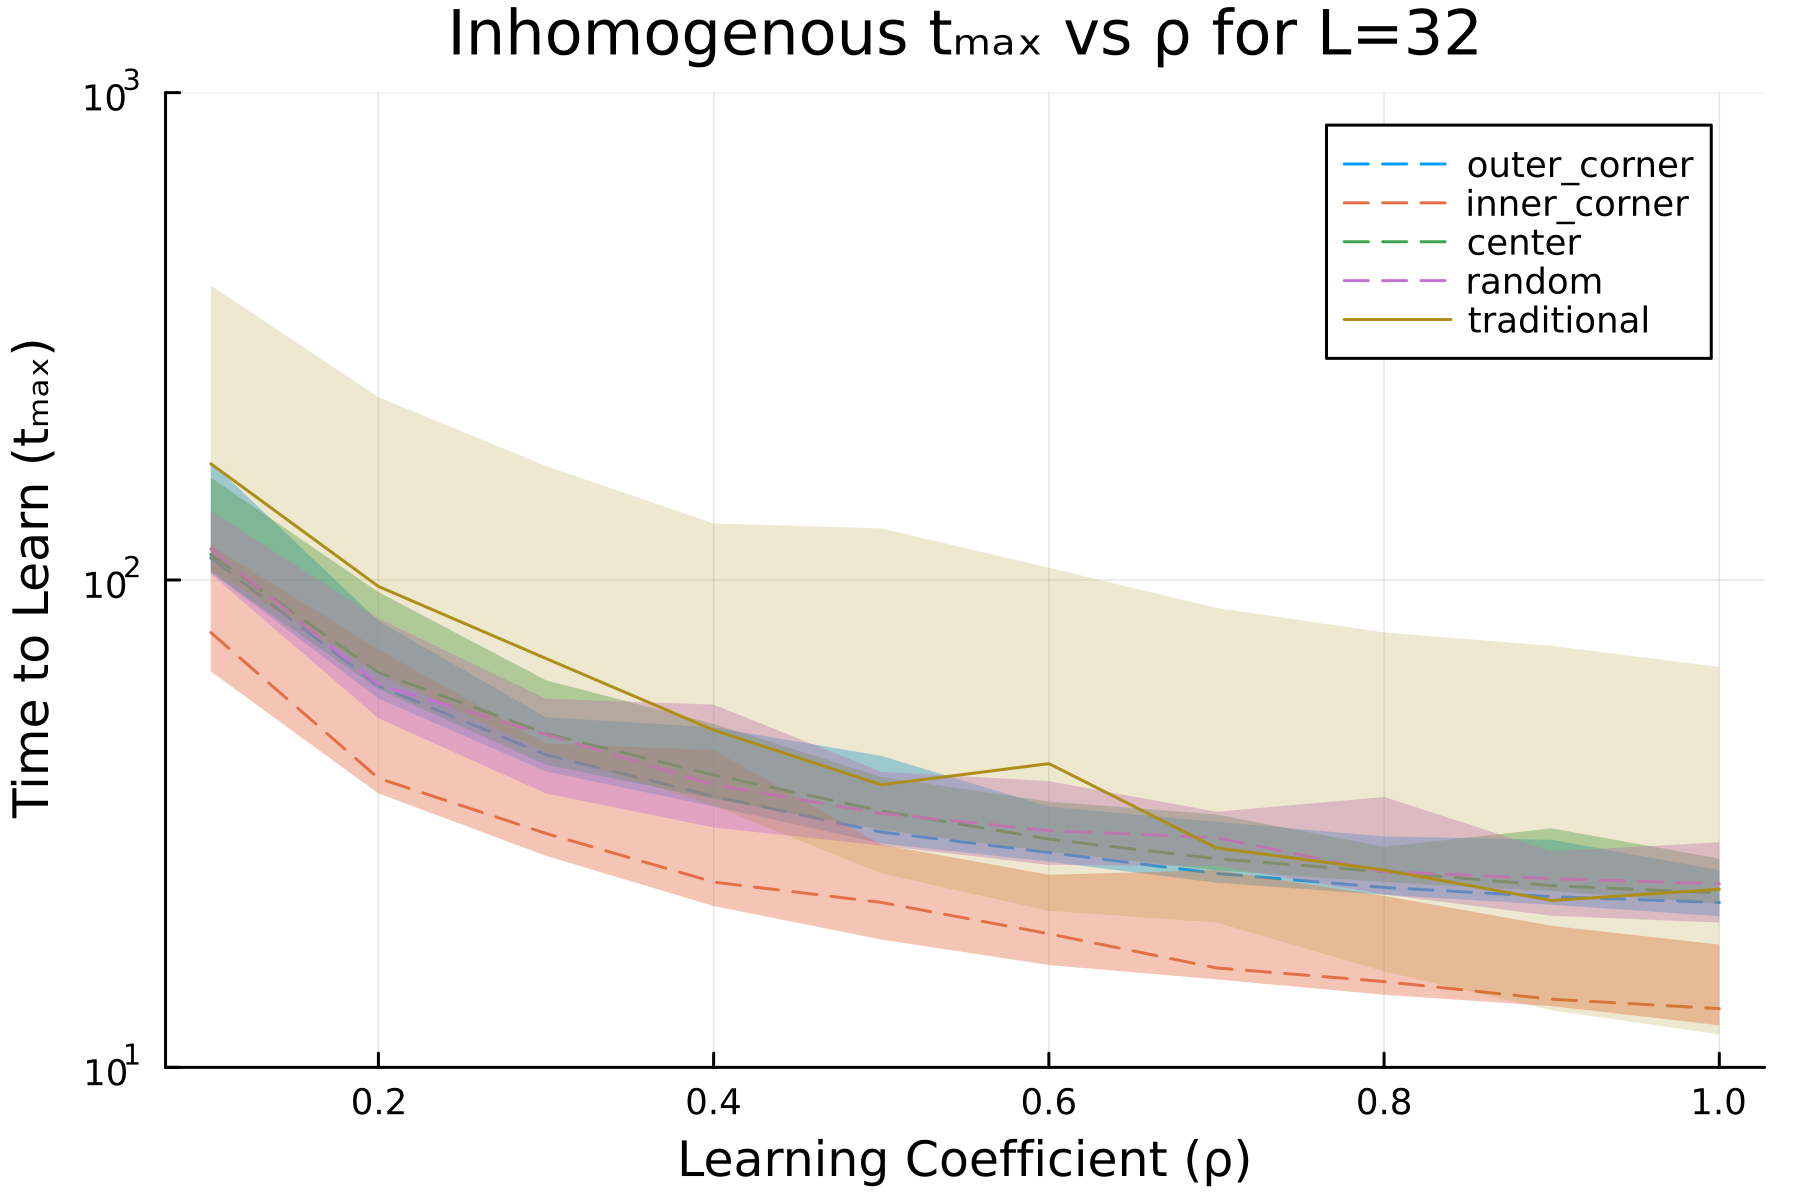
\includegraphics[width=0.49\textwidth]{figures/2D-BPCAIH-analysis/rho-t ribbon plots/rho-t-ribbon-32.png}}
    \subfigure[$L=48$]{\label{fig:2DBPCAIH t-rho ribbon plot 48}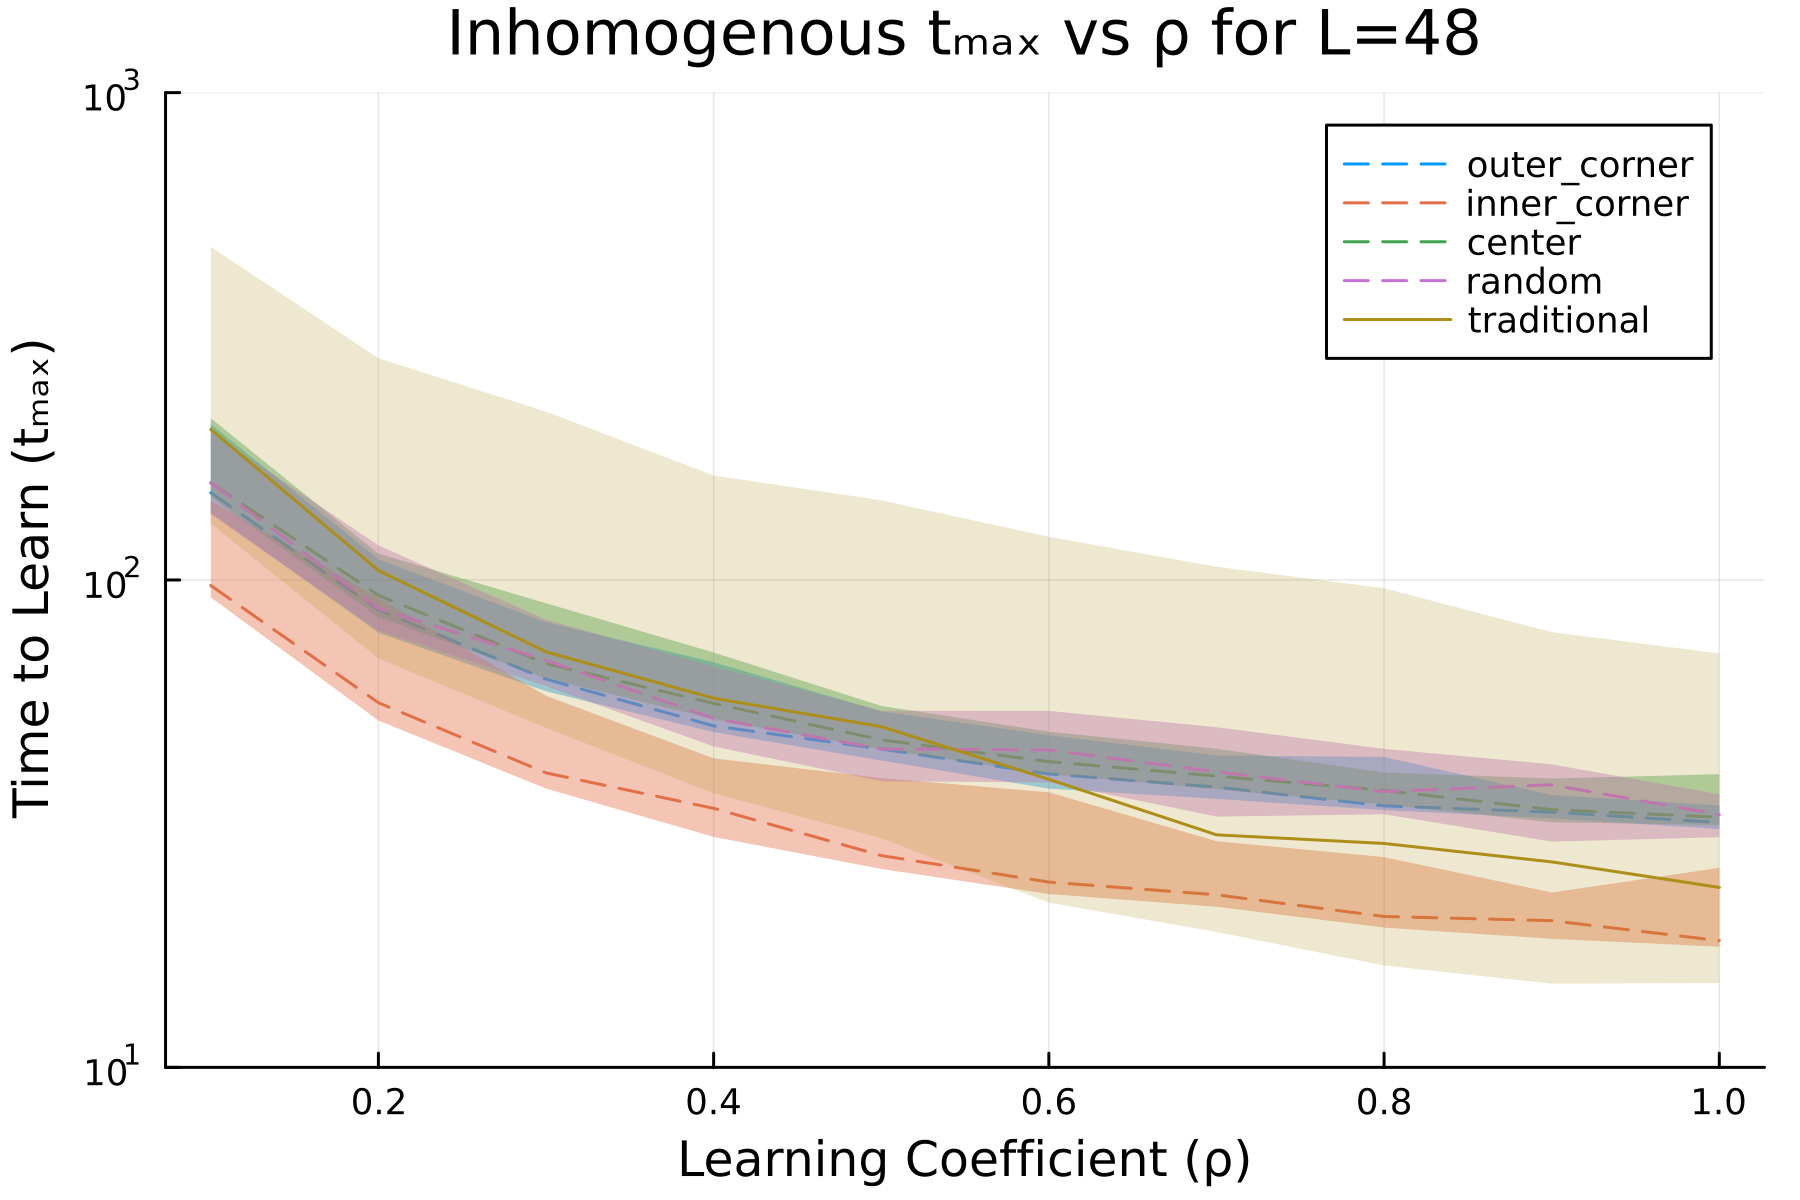
\includegraphics[width=0.49\textwidth]{figures/2D-BPCAIH-analysis/rho-t ribbon plots/rho-t-ribbon-48.png}}
    \subfigure[$L=64$]{\label{fig:2DBPCAIH t-rho ribbon plot 64}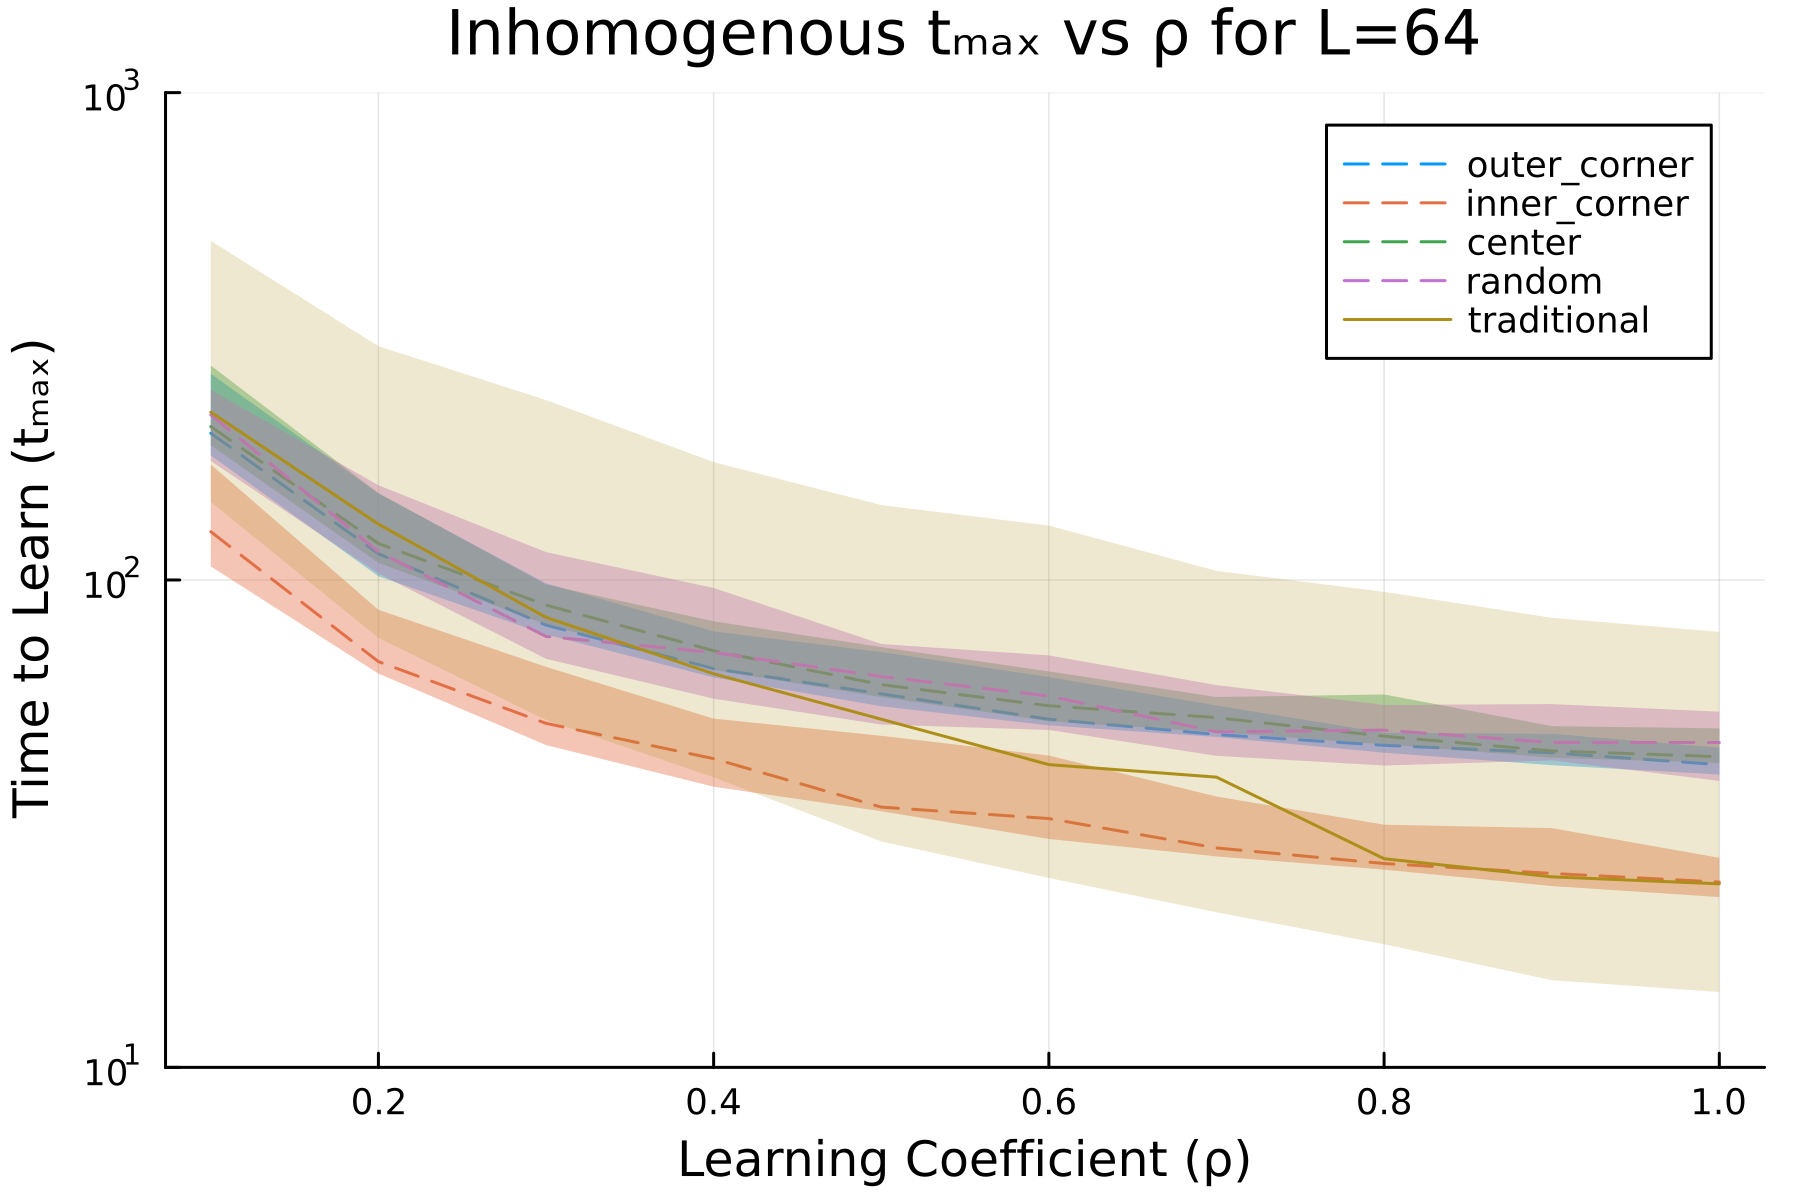
\includegraphics[width=0.49\textwidth]{figures/2D-BPCAIH-analysis/rho-t ribbon plots/rho-t-ribbon-64.png}}
    \subfigure[$L=96$]{\label{fig:2DBPCAIH t-rho ribbon plot 96}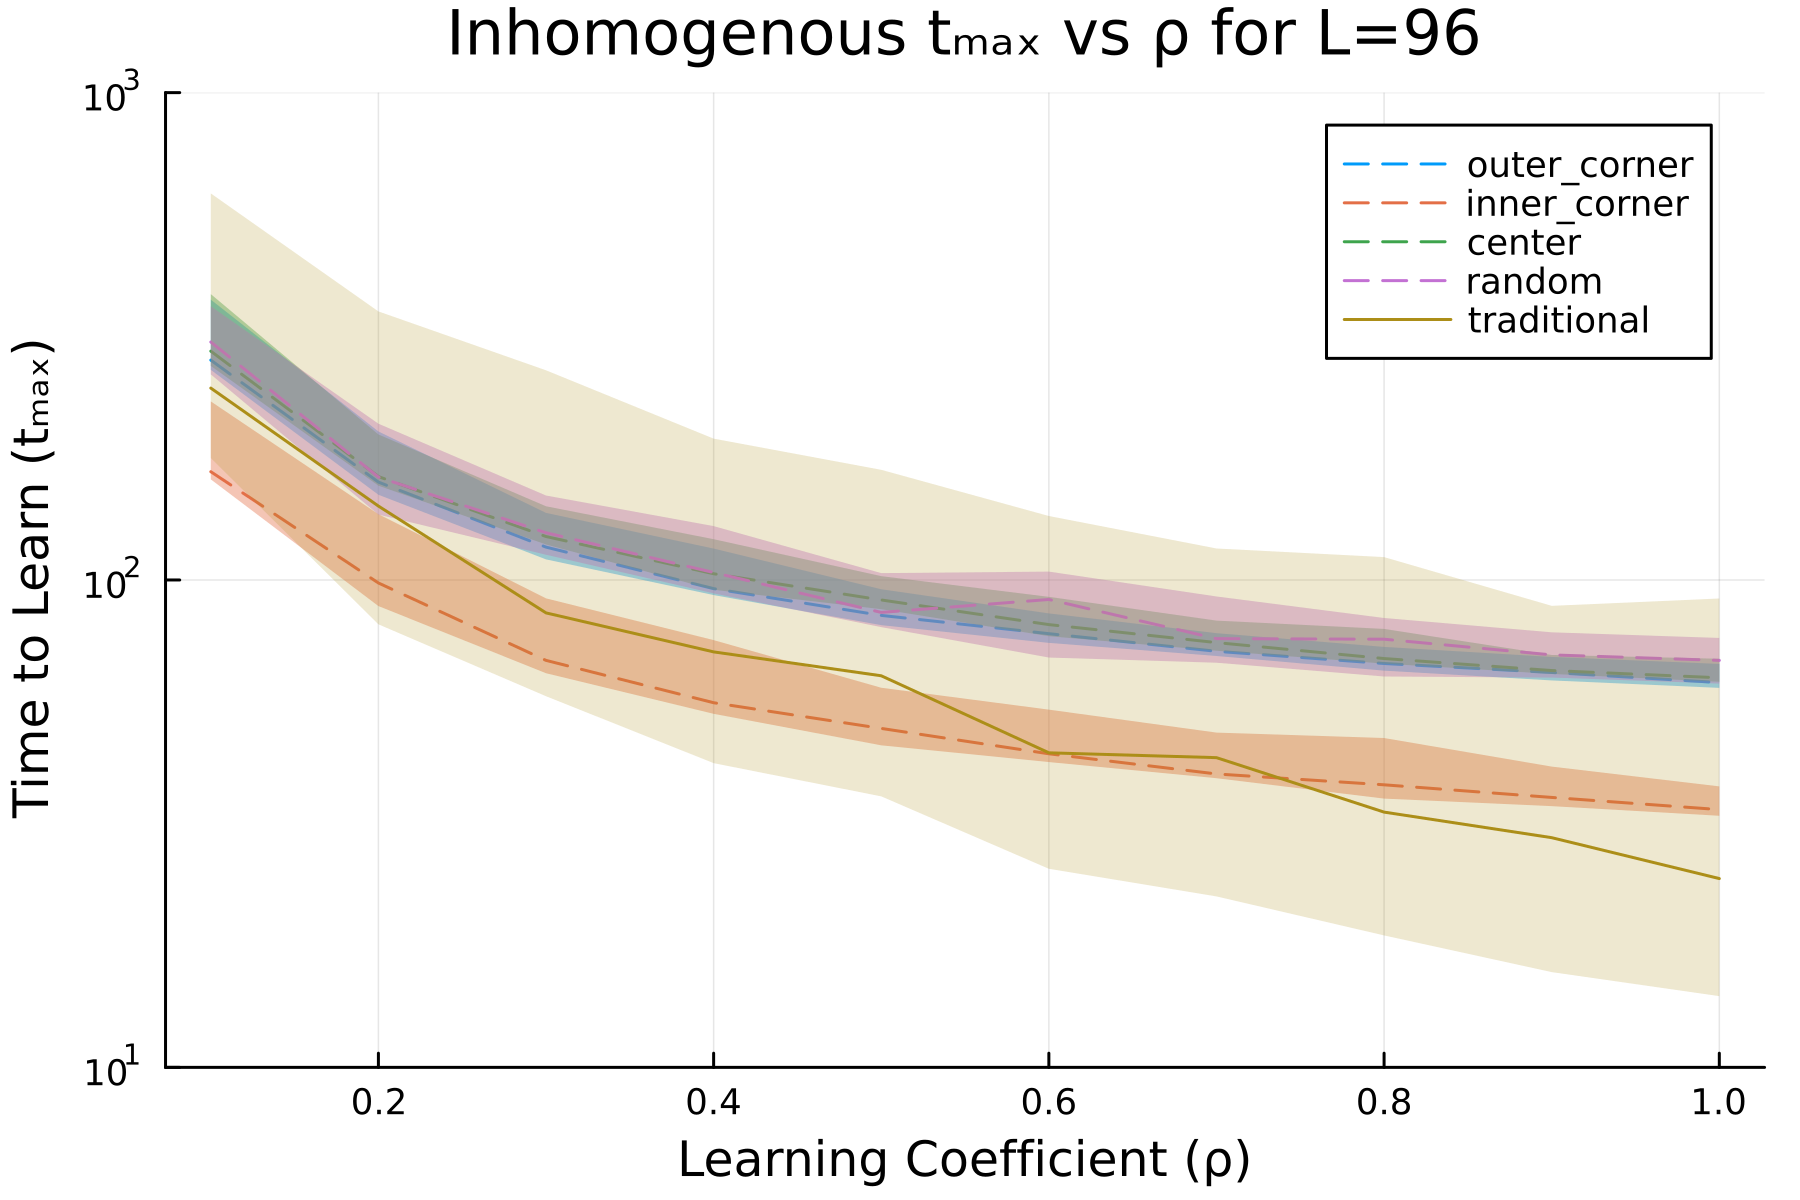
\includegraphics[width=0.49\textwidth]{figures/2D-BPCAIH-analysis/rho-t ribbon plots/rho-t-ribbon-96.png}}
    \subfigure[$L=128$]{\label{fig:2DBPCAIH t-rho ribbon plot 128}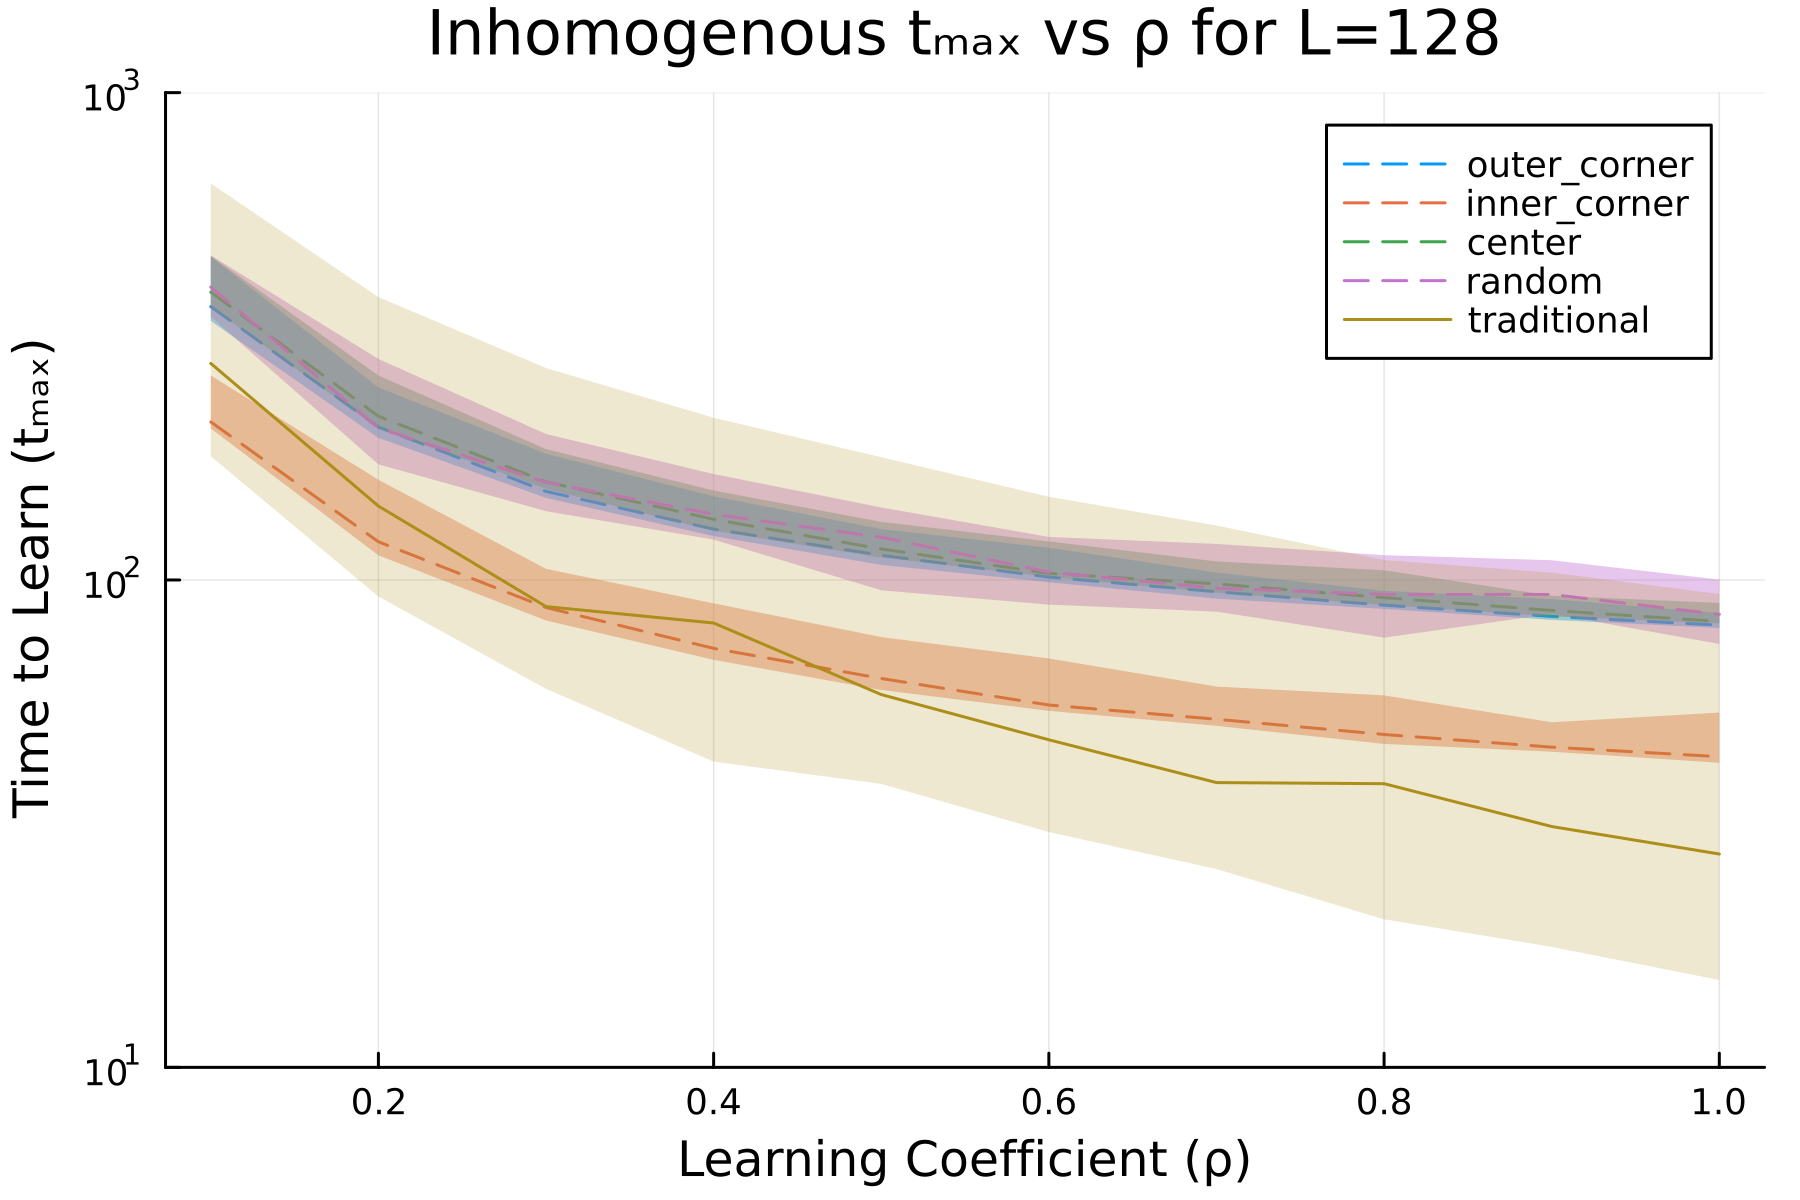
\includegraphics[width=0.49\textwidth]{figures/2D-BPCAIH-analysis/rho-t ribbon plots/rho-t-ribbon-128.png}}
    \caption{Time to learn $t_{max}$ as a function of positional learning factor $\rho_0$ for the heteregenous model of all seating arrangements and classroom sizes $L$. 
    Each ribbon series represent the range of values for $t_max$ for a given seating arrangments with heterogeneity $\delta\lambda = \lbrace 0.0, 0.1, 0.2, 0.3, 0.4 \rbrace$.
    Lower time to learn $t_{max}$ indicates better performance.
    }
    \label{fig:2DBPCAIH t-rho ribbon plot}
 \end{figure}

\subsection{$m$ vs $\delta\lambda$}\label{subsec:BPCAIH m vs dl}

\subsection{$t_{max}$ vs $\delta\lambda$}\label{subsec:BPCAIH t vs dl}

Figure \ref{fig:2DBPCAIH dl-t plots} shows that as heterogeneity $\delta\lambda$ increases, PI methods perform better than traditional methods even when PI methods have lower positional learning factors $\rho_0$. For our represntative $\rho_0$ values, PI performs better than traditional methods regardless of the $\rho_0$ value, even in a large classroom $L=128$. 
However, in larger classrooms, the advantage in performance of PI over traditional methods is less pronounced. 
Furthermore, as class size increases, traditional methods tend to stay advantageous than PI methods for increasing values of heterge $\delta\lambda$.

For example, at $L=32$ shown in figure \ref{fig:2DBPCAIH dl-t plot 32}, PI methods are better than traditional methods for all values of $\delta\lambda$ when comparing between equal $\rho_0$ values. 
However, at $L=128$ shown in figure \ref{fig:2DBPCAIH dl-t plot 128}, the traditional model performs better than the PI model for $0 \leq \delta\lambda \leq 0.2$ when comparing between equal $\rho_0$ values.

\begin{figure}[htbp!]
   \centering
   \subfigure[$L=32$]{\label{fig:2DBPCAIH dl-t plot 32}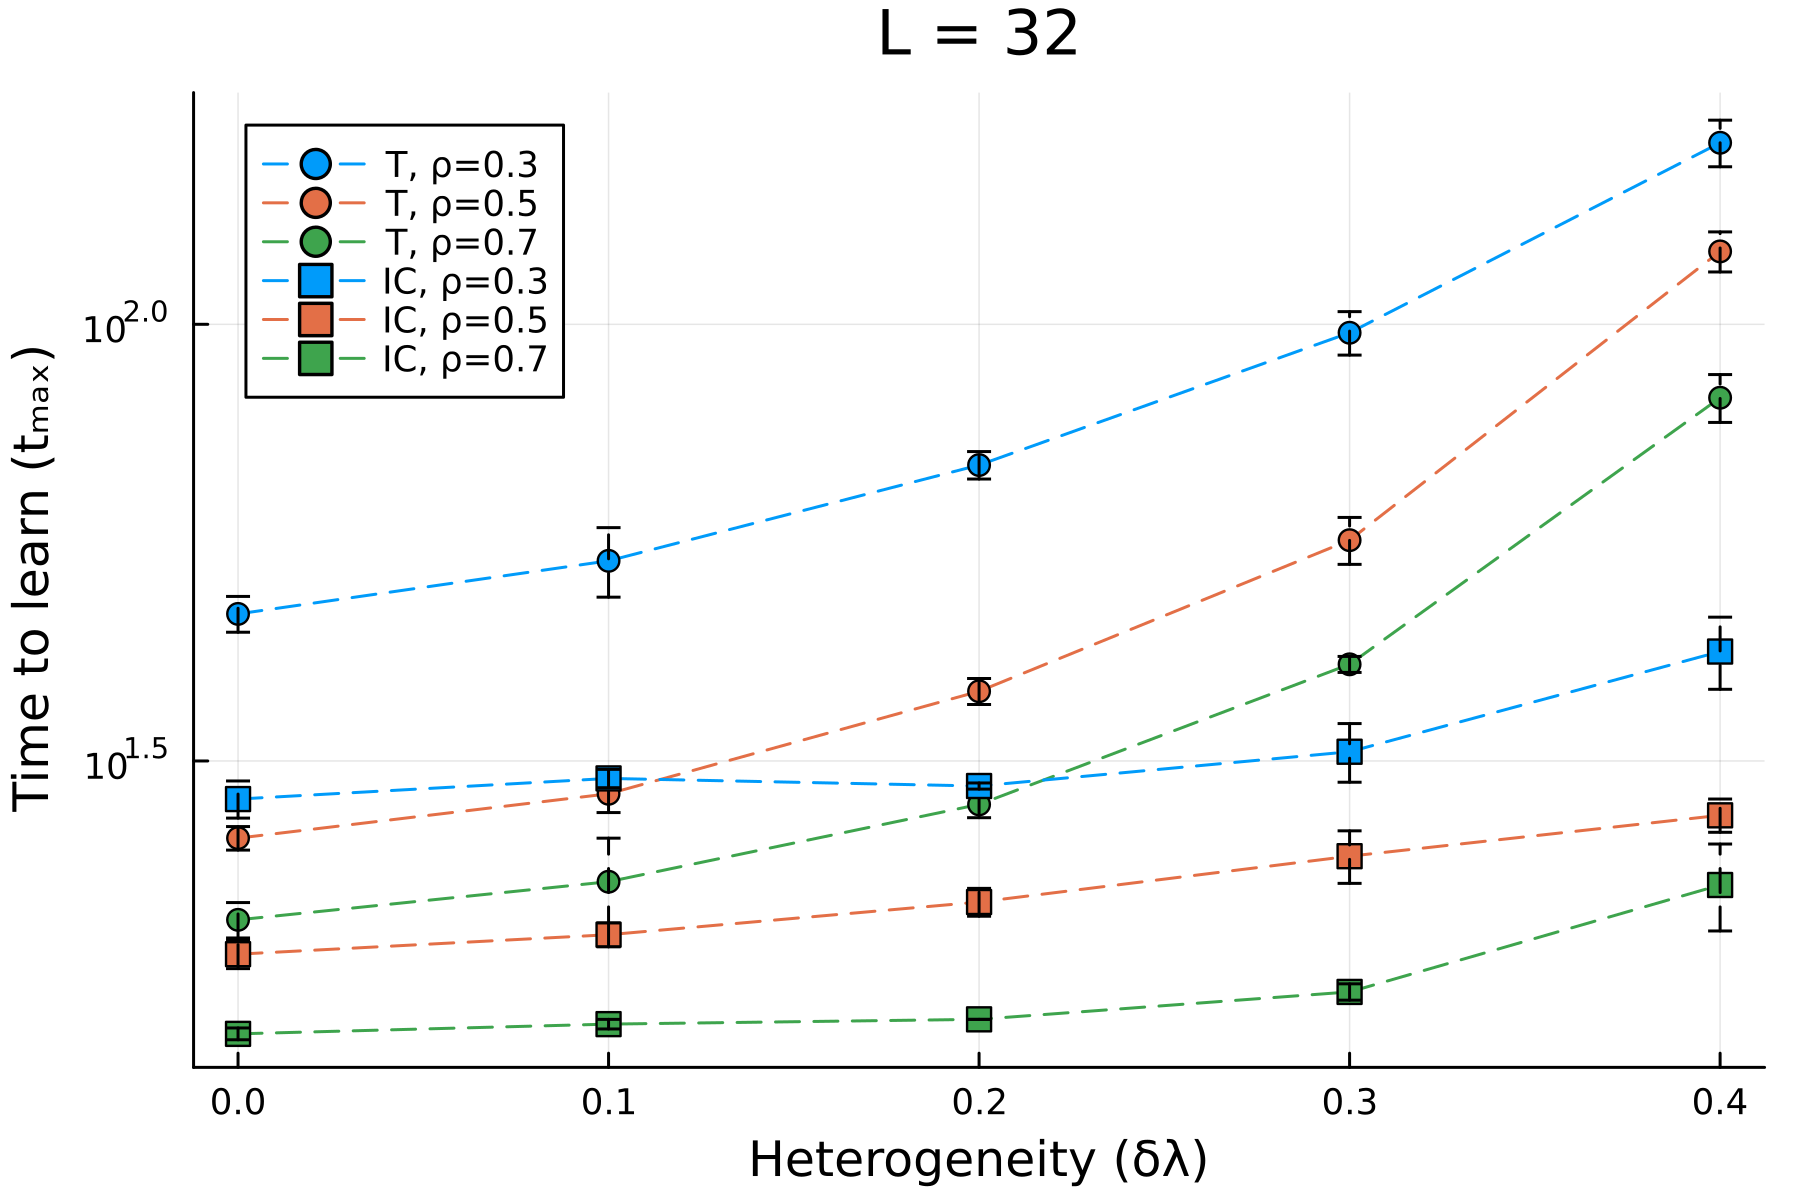
\includegraphics[width=0.49\textwidth]{figures/2D-BPCAIH-analysis/dl-t plots/dl-t-32.png}}
   \subfigure[$L=128$]{\label{fig:2DBPCAIH dl-t plot 128}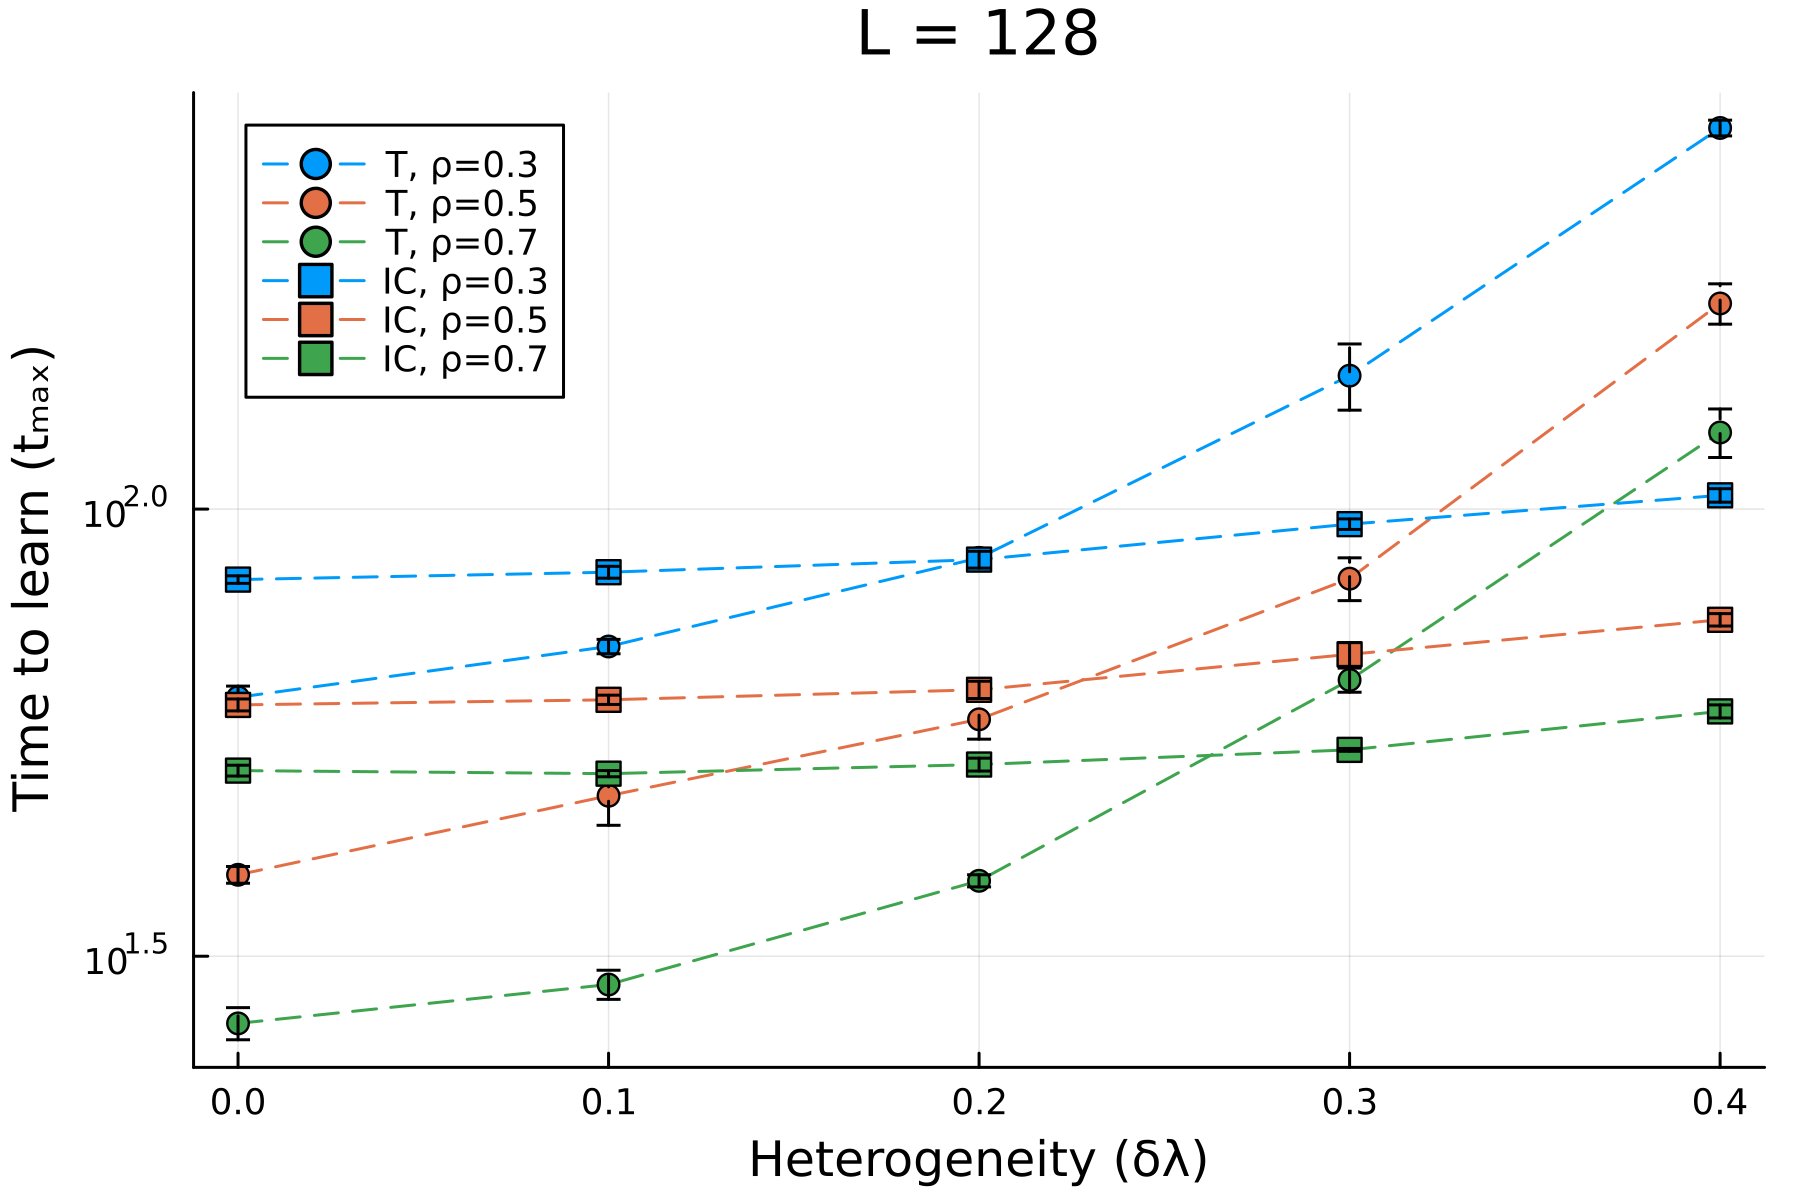
\includegraphics[width=0.49\textwidth]{figures/2D-BPCAIH-analysis/dl-t plots/dl-t-128.png}}
   \caption{Time to learn $t_{max}$ as a function of heterogeneity $\delta\lambda$ for the heteregenous models of the PI (inner corner configuration) and traditional models with varying positional learning factor $\rho_0\in\lbrace0.3,0.5,0.7\rbrace$ and classroom sizes $L\in\lbrace32,128\rbrace$. 
   Each color represents a diffent value of $\rho_0$, while the circle and square symbols represent the traditional and PI models respectively.
   Lower time to learn $t_{max}$ indicates better performance.
   }
   \label{fig:2DBPCAIH dl-t plots}
\end{figure}

\section{Anisotropic Interactions}
